\documentclass[11pt,a4paper]{article}
\usepackage[T1]{fontenc}
\usepackage[utf8]{inputenc}
\usepackage{lmodern}
\usepackage[margin=2.3cm]{geometry}
\usepackage{amsmath,amssymb,bm}
\usepackage{booktabs}
\usepackage{graphicx}
\usepackage{xcolor}
\usepackage{caption}
\usepackage{subcaption}
\usepackage{siunitx}
\usepackage{array}
\usepackage{enumitem}
\usepackage{microtype}
\usepackage[numbers,sort&compress]{natbib}
\usepackage[colorlinks=true,linkcolor=blue!50!black,citecolor=blue!50!black,urlcolor=blue!50!black]{hyperref}
\usepackage{url}
\graphicspath{{figures/}}
\captionsetup{font=small,labelfont=bf}
\setlist{itemsep=2pt,topsep=4pt}
\newcommand{\R}{\mathbb{R}}

\title{\textbf{Climate-Aware Stochastic Optimization of Hydropower, Renewable Generation, and Battery Storage for Electricity-System Resilience in Albania}}
\author{Ajsel Budlla\\[2pt]
\small Whitman College, Walla Walla, Washington, USA\\
\small \textit{Research prototype — preprint, not peer reviewed}}
\date{\small Manuscript generated from the HYDROFLEX AI experiment pipeline}

\begin{document}
\maketitle

\begin{abstract}
\noindent Albania generates almost all of its electricity from hydropower, so rainfall variability translates
directly into import dependence. We present HYDROFLEX AI, an open and reproducible linear-programming model
that coordinates a physically explicit reservoir water balance, run-of-river hydro, solar, wind, batteries
with independent power and energy sizing, and a capacity-limited interconnector. It is solved with the open
HiGHS solver and verified against an independent PyPSA formulation (objectives agree to solver precision). The planning layer is a two-stage stochastic programme with a conditional-value-at-risk (CVaR)
term, built on hourly representative weeks whose seasonal boundaries are valued at water values from a coarse
annual model. The planning results were checked against full-year chronology: representative-week costs are
within 1.7--10~MEUR/yr, and the strategies rank in the same order. Inputs are weather-derived capacity
factors (NASA POWER), reconstructed inflows and \emph{synthetic} demand and prices.

\noindent With a fully available interconnector, a 40\% inflow reduction causes no shortage but raises net
imports from 0.8 to 3.5~TWh/yr and operating cost by 284~MEUR/yr. Shortages appear only when import
availability falls to about half, and they are energy-limited. In that regime batteries pay for themselves
through avoided unserved energy, but not through arbitrage alone (13--27\% of their cost). Solar PV is a
no-regret investment under the base assumptions: its marginal value is about 140~kEUR/MW-yr against an
80~kEUR/MW-yr cost. Because PV dominates, stochastic and risk-averse planning select the same plan as
deterministic planning (value of the stochastic solution = 0). When exports are restricted to 300~MW,
risk-averse planning adds wind and cuts CVaR$_{0.9}$ by 74.5~MEUR/yr for 15.1~MEUR/yr of expected cost
(full-year chronology). Coarse time steps and pinned week boundaries each distorted the conclusions. The model
has not been validated against observed Albanian operations.
\end{abstract}

\section{Introduction}
\label{sec:intro}

Albania is one of the most hydropower-dependent electricity systems in Europe. Hydropower made up about
95\% of installed generating capacity at the end of 2018 (2{,}096~MW), and the River Drin cascade, made up of
Fierza (500~MW), Koman (600~MW) and Vau i Dejës (250~MW), is the backbone of domestic supply
\cite{irena2021rra,kesh2026drin}. This structure makes annual electricity supply a function of rainfall and
snowmelt. Reported net imports are closely correlated with annual precipitation \cite{irena2021rra}, and
IRENA's assessment projects that average output from large and small hydropower plants could be roughly 15\% and
20\% lower by 2050 than in 2010 \cite{irena2021rra}. Climate variability is therefore not a remote planning
consideration for Albania. It is the dominant operational risk.

Three developments make the question of \emph{flexibility} timely. First, utility-scale solar photovoltaics
(PV) and batteries have become much cheaper; IRENA reports global weighted-average installed costs of
USD~691/kW for PV, USD~1{,}041/kW for onshore wind and USD~192/kWh for battery storage projects in 2024
\cite{irena2025costs}. Second, the reservoir fleet is itself a large energy store whose seasonal value
depends on how it is coordinated with variable renewables and imports \cite{labadie2004reservoir}. Third,
regional interconnections let a hydro system import in dry periods and export in wet ones. That exposes
the system to regional prices and to the availability of transfer capacity.

This paper asks: \emph{how should a hydropower-dependent electricity system coordinate reservoir operation,
renewable generation, battery storage and electricity imports under uncertain rainfall, fluctuating demand
and financial constraints?} We address eight supporting questions. They cover the reliability effect of
drought, the import-reduction potential of solar, wind and batteries, how storage value changes with drought
severity, budget-constrained investment, the performance of plans optimised for average conditions under
shocks, the value of stochastic and risk-averse planning, the marginal value of each flexibility resource, and
sensitivity to prices, demand, costs and inflows.

\paragraph{Contributions.} The work is an independent research prototype with four contributions:
\begin{enumerate}
\item An open, fully reproducible linear-programming model of the Albanian system. It couples an hourly
energy balance with a physically consistent reservoir water balance (in hm$^3$, with an explicit energy
equivalent), independent battery power and energy sizing, an aggregate interconnector and an unserved-energy
penalty. It is solved with the open-source HiGHS solver and verified against an independent PyPSA formulation.
\item A two-stage stochastic investment programme with a Rockafellar--Uryasev CVaR term. Capacities are
shared first-stage decisions and dispatch is scenario specific at hourly resolution on representative weeks.
Seasonal reservoir coupling is retained through nested annual boundary conditions.
\item A transparent climate-scenario construction that ties drought severities to a reconstructed
2001--2023 inflow index derived from NASA POWER precipitation. Every series is labelled as weather-derived,
reconstructed or synthetic.
\item A systematic marginal-value analysis that compares dual-based and finite-difference values of
battery energy, battery power, PV, wind, import capacity and reservoir volume, and states explicitly when
duals can and cannot be interpreted economically.
\end{enumerate}
The model is embedded in an interactive decision-support application whose numbers come exclusively from
executed optimisation runs. We stress at the outset what the work is not. It is not an operational model,
it has not been validated against observed Albanian grid operations, and its demand and price inputs are
synthetic (Section~\ref{sec:limitations}).

\section{Literature review}
\label{sec:lit}

\paragraph{Hydropower-dependent systems and climate risk.}
Hydro-dominated systems face supply risk that is driven by water availability rather than by generating
capacity. At the global scale, van Vliet et al.\ \cite{vanvliet2016vulnerability} showed that a large share of
hydropower and thermoelectric capacity is vulnerable to reduced streamflow and warmer water under climate change.
They also argued that adaptation options such as efficiency gains and fuel switching matter. For Albania,
IRENA's readiness assessment highlights both the dominance of the Drin cascade and the projected decline in
hydro output \cite{irena2021rra}. Reservoir operation has a long literature of its own
\cite{labadie2004reservoir}. Stochastic dual dynamic programming (SDDP) \cite{pereira1991sddp} remains the
reference method for multi-stage hydrothermal scheduling under inflow uncertainty. We use a simpler two-stage
structure that is adequate for investment screening (Section~\ref{sec:formulation}), and we note SDDP as a
natural extension.

\paragraph{Renewable capacity expansion and open models.}
Linear capacity-expansion models that co-optimise investment and hourly dispatch are standard tools
\cite{pfenninger2014modeling}. PyPSA \cite{brown2018pypsa} and its European application PyPSA-Eur
\cite{horsch2018pypsaeur} established open, reproducible practice for such models. Studies with them have
shown, for example, the value of transmission cooperation in highly renewable systems
\cite{schlachtberger2017cooperation}. Weather-derived capacity factors from reanalysis are widely used when
measured output is unavailable. They require care, however, because reanalysis wind speeds are biased and
need correction at the site level \cite{staffell2016wind,pfenninger2016pv,gelaro2017merra2,hersbach2020era5}.

\paragraph{Flexibility and storage.}
Reviews of flexibility options \cite{lund2015flexibility,kondziella2016flexibility} distinguish short-duration
resources (batteries, demand response) from long-duration ones (reservoir hydro, interconnection). The value
of short-duration storage depends strongly on the temporal resolution of the model: coarse time steps average
away the intra-day variability that storage monetises \cite{poncelet2016temporal}. Representative-period
methods reduce computation but must treat seasonal storage carefully \cite{kotzur2018seasonal}. Projected
storage costs continue to fall \cite{schmidt2019storage}. The market value of variable renewables declines as
their penetration rises \cite{hirth2013market}, which is directly relevant to solar-heavy expansion in a
small system.

\paragraph{Stochastic and risk-sensitive planning.}
Two-stage stochastic programming \cite{birge2011stochastic} separates here-and-now investment from
wait-and-see operation. The value of the stochastic solution (VSS) and the expected value of perfect
information (EVPI) quantify, respectively, the benefit of modelling uncertainty and the cost of not knowing
the future \cite{birge2011stochastic,madansky1960inequalities}. Conditional value at risk (CVaR) admits a
linear representation \cite{rockafellar2000cvar,rockafellar2002cvar} and is widely used in electricity
decision problems \cite{conejo2010decision}. Reliability is commonly priced through a value of lost load
(VOLL), whose empirical estimates vary by an order of magnitude across countries and customer groups
\cite{schroder2015voll}. This motivates the sensitivity analysis reported below.

\paragraph{Gap.}
We are not aware of an open, reproducible model of Albania that combines (i)~a physically explicit reservoir
water balance, (ii)~independent battery power and energy investment, (iii)~an interconnector that is limited
rather than infinite, (iv)~two-stage stochastic investment with CVaR, and (v)~a marginal-value analysis of
flexibility with dual--finite-difference reconciliation. This work offers such a model as a transparent
research prototype.

\section{Data and study context}
\label{sec:data}

\paragraph{Scope.} The study area is Albania, represented as a single node with an aggregate interconnector to
its neighbours (Fig.~\ref{fig:context}). All series are indexed in UTC. Local time (Europe/Tirane) is used only to
shape behavioural demand and price patterns. Monetary values are in 2024 euros, converted from USD at
0.92~EUR/USD. Energies are in MWh, powers in MW and water volumes in hm$^3$.

\begin{figure}[htbp]
\centering
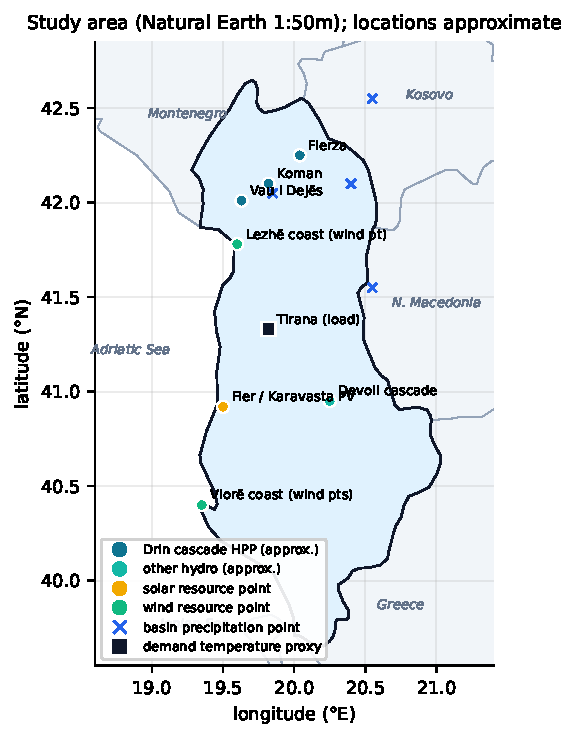
\includegraphics[width=0.48\textwidth]{fig02_study_context.pdf}
\caption{Study area. The Albanian boundary and its neighbours are from Natural Earth 1:50m \cite{naturalearth2026}. Plant
locations are approximate and shown only for orientation; the model itself has no spatial resolution. Crosses
are the four NASA POWER points used to compute basin-mean precipitation for the Drin inflow
reconstruction. Coloured circles are the PV and wind resource points.}
\label{fig:context}
\end{figure}

\paragraph{Meteorological inputs (observed-derived).} Hourly all-sky irradiance, 2-m temperature and 50-m wind
speed for 2019--2023 were retrieved from the NASA POWER point API \cite{nasapower2026} for five points: two
solar (Fier/Myzeqe, Vlorë), two coastal wind (Vlorë--Karaburun, Lezhë--Shëngjin) and a Tirana demand
proxy. Daily bias-corrected precipitation and temperature for 2000--2023 were retrieved for four points in the
Drin basin (White Drin, Black Drin, Kukës/Fierza, Koman). Open-Meteo ERA5 data for Tirana in 2021
\cite{openmeteo2026} were retrieved as a cross-check only. Every dataset has a machine-readable provenance
record (Table~\ref{tab:data-dictionary} in the Appendix).

\paragraph{PV and wind capacity factors (weather-derived).} PV output follows a simplified PVWatts-type model
\cite{dobos2014pvwatts}: horizontal irradiance with a constant tilt gain of 1.10, system losses of 0.86 and a
temperature derating of $-0.4\%/^\circ$C, with cell temperature estimated from a nominal operating cell
temperature (NOCT) of $45^\circ$C. Wind output scales the 50-m wind speed to a 100-m hub height using a shear
exponent of 0.14 and applies a generic 3/12/25~m/s power curve with 0.85 losses. The mean annual capacity
factors are 0.170--0.176 for PV and 0.108--0.119 for wind across 2019--2023. The wind values are low, and are
likely conservative because coarse reanalysis smooths coastal and orographic winds \cite{staffell2016wind}.
These are modelled availabilities, \emph{not measured production}.

\paragraph{Hydrology (reconstructed).} Basin-mean precipitation and temperature drive a degree-day snow model
\cite{hock2003melt} (threshold $0.5^\circ$C, 3~mm/$^\circ$C/day). Its output feeds two parallel linear
reservoirs \cite{beven2012rainfall} with recession constants of 4 and 45 days. The resulting runoff index is
scaled so that the 2001--2023 mean inflow volume yields an \emph{assumed} long-run Drin-cascade energy of
4.1~TWh/yr. This is consistent in magnitude with the reported mean output of about 1.33~TWh for Fierza alone,
the uppermost of the three stages. Run-of-river availability for the remaining hydro fleet (about 930~MW,
Table~\ref{tab:assumptions}) is a normalised blend of fast and total runoff, capped at capacity and scaled to
2.6~TWh/yr. No gauge or plant records were accessible, so the hydrological parameters are uncalibrated
assumptions. The reconstructed annual inflow index (Fig.~\ref{fig:profiles}d) has a 5th percentile of 0.78, a
median of 0.99 and a minimum of 0.67 (2011). The reference weather year, 2022, was selected algorithmically as
the 2019--2023 year closest to the median. This ranking should not be read as the observed hydrology of 2022.

\paragraph{Demand and prices (synthetic).} ENTSO-E Transparency data require a registered token, which was not
used. Hourly demand is therefore \textbf{synthetic}. It is generated from Tirana temperature with assumed
heating (3.0\%/$^\circ$C below $16^\circ$C) and cooling (3.5\%/$^\circ$C above $24^\circ$C) sensitivities, an
assumed diurnal and weekly shape, and AR(1) noise with a fixed seed, and it is scaled to an assumed
8.0~TWh/yr. Its peak is about 1.64~GW. Import prices are also synthetic: the mean is 105~EUR/MWh, with diurnal
and seasonal shapes and multiplicative AR(1) noise. Export revenue is 85\% of the import price, which
represents transmission charges and market spreads. All outputs carry the label \emph{``synthetic research
demonstration data --- not observed grid operations''}.

\begin{figure}[htbp]
\centering
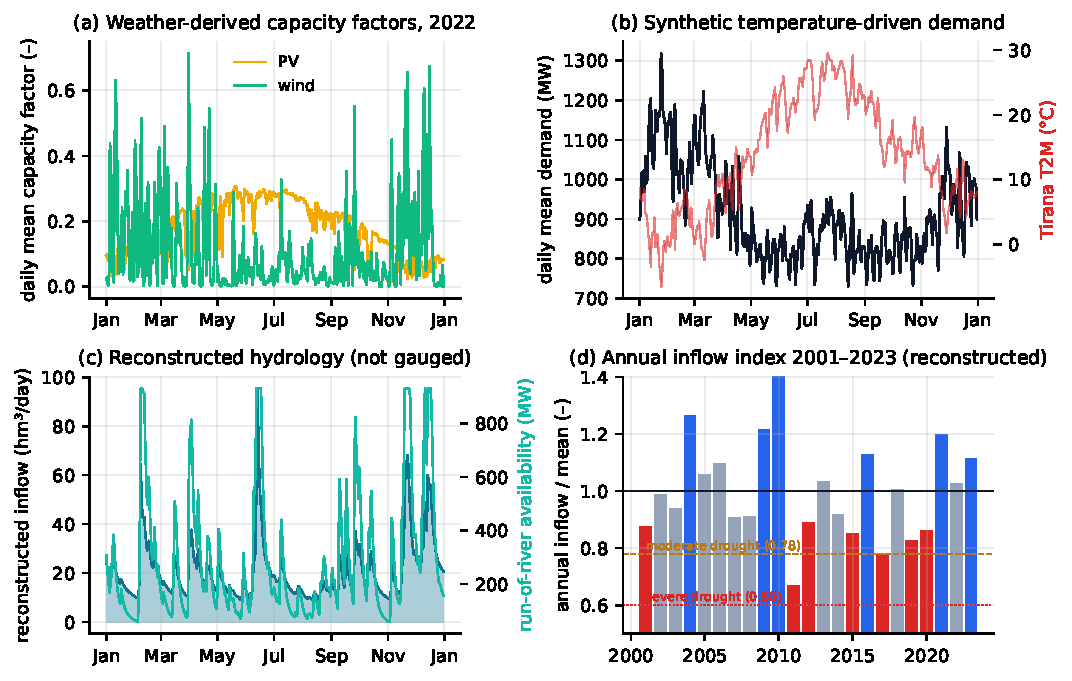
\includegraphics[width=\textwidth]{fig03_profiles.pdf}
\caption{Model inputs for the reference year. (a)~Daily mean PV and wind capacity factors derived from NASA POWER.
(b)~Synthetic temperature-driven demand. (c)~Reconstructed Drin inflow and run-of-river availability.
(d)~Reconstructed annual inflow index for 2001--2023 relative to its mean, with the moderate (0.78) and severe
(0.60) drought scenario levels marked.}
\label{fig:profiles}
\end{figure}

\paragraph{System and cost parameters.} Table~\ref{tab:assumptions} lists all key parameters and their status.
Sourced values are the Drin cascade capacities \cite{kesh2026drin}, the hydro fleet size \cite{irena2021rra} and
the IRENA 2024 technology costs \cite{irena2025costs}. We apply an assumed regional cost multiplier of 1.25
because global weighted averages are dominated by low-cost markets. The remaining values are assumptions
chosen to be of plausible magnitude, and the important ones are varied in Section~\ref{sec:sensitivity}.

\begin{table}[htbp]
\centering
\footnotesize
\caption{Key system and cost parameters. ``Assumption'' marks values chosen for this study that were not taken from an observed Albanian dataset.}
\label{tab:assumptions}
\begin{tabular}{p{5.2cm}lrp{5.0cm}}
\toprule
Parameter & Unit & Value & Source / status \\
\midrule
Drin cascade turbine capacity & MW & 1\,350 & KESH (Fierza 500, Koman 600, Vau i Dejës 250) \\
Aggregate head / efficiency & m / -- & 230 / 0.88 & assumption \\
Energy equivalent $\kappa$ & MWh/hm$^3$ & 551.5 & derived \\
Reservoir $V^{\min}$ / $V^{\max}$ & hm$^3$ & 600 / 2400 & assumption \\
Initial volume (live fraction) & -- & 0.60 & assumption \\
Minimum release & m$^3$/s & 20 & assumption \\
Other hydro (run-of-river aggregate) & MW & 930 & IRENA RRA (2,096 MW, 2018) + Moglicë 184 MW $-$ Drin \\
Existing PV / wind & MW & 300 / 0 & assumption (order of magnitude) \\
Import / export NTC & MW & 900 / 900 & assumption \\
Export price ratio $\rho$ & -- & 0.85 & assumption \\
VOLL & EUR/MWh & 5\,000 & assumption (varied 2,000--10,000) \\
Battery $\eta^c$, $\eta^d$ / min SOC & -- & 0.95, 0.95 / 0.05 & assumption \\
Battery degradation proxy & EUR/MWh & 5.0 & assumption \\
PV capex (incl. ×1.25 regional) & EUR/kW & 795 & IRENA RPGC 2024: USD 691/kW \\
Onshore wind capex (incl. ×1.25) & EUR/kW & 1\,197 & IRENA RPGC 2024: USD 1,041/kW \\
Battery energy capex (incl. ×1.25) & EUR/kWh & 221 & IRENA RPGC 2024: USD 192/kWh \\
Battery power capex (incl. ×1.25) & EUR/kW & 75 & assumption \\
Discount rate / lifetimes & -- / yr & 0.07 / 25, 25, 15 & assumption \\
Annualised PV / wind & kEUR/MW-yr & 80.1 / 132.7 & derived (CRF + FOM) \\
Annualised battery power / energy & kEUR/(MW, MWh)-yr & 10.1 / 29.8 & derived \\
\bottomrule
\end{tabular}
\end{table}


\paragraph{Scenarios.} Each scenario applies a transparent transformation to the reference-year profiles.
Inflows are scaled by $(1-d)$, demand by $(1+g)$ and import prices by $m$, and interconnector availability
is set to $a$ (Table~\ref{tab:scenarios}). The \emph{moderate drought} ($d=0.22$) corresponds to the 5th
percentile of the reconstructed inflow index. The \emph{severe drought} ($d=0.40$) lies beyond the
reconstructed minimum and represents a climate-stress extrapolation. The \emph{compound shock} adds 8\% demand
growth, a 1.8$\times$ import-price shock and a 30\% derating of transfer capacity, all assumed. For two-stage
planning, five scenarios are used. Three come from binning the 23 reconstructed years (wet $>1.10$, normal
0.90--1.10, dry $<0.90$), with their empirical frequencies scaled to 85\% of the probability mass. The other
two are the severe and compound stresses, with an assumed 10\% and 5\%. These probabilities are partly assumed
and are reported as such.

\begin{table}[htbp]
\centering
\small
\caption{Climate and market scenarios. Upper block: named stress presets; lower block: five-scenario set for two-stage planning (historical-bin probabilities from the reconstructed 2001--2023 inflow index, plus an assumed 15\% climate-stress allowance).}
\label{tab:scenarios}
\begin{tabular}{lrrrrr}
\toprule
Scenario & Inflow factor & Demand factor & Import price & NTC avail. & Prob. \\
\midrule
Normal & 1.00 & 1.00 & 1.00 & 1.00 & -- \\
Moderate drought & 0.78 & 1.00 & 1.00 & 1.00 & -- \\
Severe drought & 0.60 & 1.00 & 1.00 & 1.00 & -- \\
Compound shock & 0.60 & 1.08 & 1.80 & 0.70 & -- \\
Wet year (stoch.) & 1.226 & 1.00 & 1.00 & 1.00 & 0.222 \\
Normal (stoch.) & 0.989 & 1.00 & 1.00 & 1.00 & 0.370 \\
Dry year (stoch.) & 0.823 & 1.00 & 1.00 & 1.00 & 0.259 \\
Severe drought (stoch.) & 0.600 & 1.00 & 1.00 & 1.00 & 0.100 \\
Compound shock (stoch.) & 0.600 & 1.08 & 1.80 & 0.70 & 0.050 \\
\bottomrule
\end{tabular}
\end{table}


\section{Mathematical formulation}
\label{sec:formulation}

\subsection{Sets, decisions and parameters}
Let $\mathcal{T}=\{0,\dots,T-1\}$ be time steps of length $\Delta t$ (h) and $\mathcal{S}$ the scenarios, each with
probability $\pi_s$. First-stage decisions $x=(x_{pv},x_{w},x_{bp},x_{be})$ are the installed PV and wind
capacity (MW), battery power (MW) and battery energy (MWh). Each satisfies
$x_k^0\le x_k\le x_k^0+\bar x_k$, where $x_k^0$ is the existing fleet and $\bar x_k$ the maximum addition. Import
capacity $x_{imp}$ (MW) and maximum reservoir volume $x_{vmax}$ (hm$^3$) are modelled as fixed first-stage
variables ($x_k=x_k^0$). This lets their reduced costs be read as marginal values (Section~\ref{sec:marginal}).
Second-stage decisions for each $(s,t)$ are the PV, wind and run-of-river generation $g^{pv},g^{w},g^{ror}$, the
reservoir hydro output $h$, spill $\sigma$ (hm$^3$/h), reservoir volume $V$ (hm$^3$), battery charge $c$,
discharge $d$ and state of charge $e$, imports $m$, exports $y$ and unserved energy $u$. All are non-negative.

\subsection{Objective}
\begin{equation}
\min\; w\sum_{k\in\{pv,w,bp,be\}} A_k\,(x_k-x_k^0)\;+\;\sum_{s}\pi_s L_s\;+\;\lambda\Big[\zeta+\frac{1}{1-\alpha}\sum_s\pi_s\phi_s\Big],
\label{eq:obj}
\end{equation}
\begin{equation}
L_s=\frac{1}{1000}\sum_{t}\Delta t\,\Big(p^m_{s,t}m_{s,t}-\rho\,p^m_{s,t}y_{s,t}+\mathrm{VOLL}\,u_{s,t}+c^h h_{s,t}+c^{\deg}d_{s,t}\Big)\quad\text{(kEUR)},
\label{eq:opex}
\end{equation}
\begin{equation}
\phi_s\ge L_s-\zeta,\qquad \phi_s\ge0,\qquad \zeta\in\R .
\label{eq:cvar}
\end{equation}
Here $A_k=C_k[\,r(1+r)^{n_k}/((1+r)^{n_k}-1)+f_k\,]$ is the annualised cost per unit, combining the capital
recovery factor with fixed O\&M as a share $f_k$ of overnight cost $C_k$. The factor $w=T\Delta t/8760$ scales
annual costs to the modelled horizon. Existing capacity is sunk and therefore not charged. The remaining
parameters are the import price $p^m$, the export-to-import price ratio $\rho$, hydro variable O\&M $c^h$ and a
battery throughput degradation proxy $c^{\deg}$. At the optimum, $\zeta$ equals the value at risk $\mathrm{VaR}_\alpha$
of the operating-cost distribution, and the bracketed term equals $\mathrm{CVaR}_\alpha$
\cite{rockafellar2000cvar,rockafellar2002cvar}. With $\lambda=0$ the model is risk neutral; with $\lambda>0$ it
penalises the expected cost of the worst $(1-\alpha)$ tail. Investment cost is identical across scenarios, so
the risk term acts on operating cost.

\subsection{Constraints}
\paragraph{Energy balance.} For every $(s,t)$, whose dual is the system marginal cost:
\begin{equation}
g^{pv}_{s,t}+g^{w}_{s,t}+g^{ror}_{s,t}+h_{s,t}+d_{s,t}+m_{s,t}+u_{s,t}=D_{s,t}+c_{s,t}+y_{s,t}.
\label{eq:balance}
\end{equation}
Curtailment is implicit: $g^{pv}_{s,t}\le f^{pv}_t x_{pv}$ and $g^{w}_{s,t}\le f^{w}_t x_{w}$, so curtailed energy is
$f^{pv}_t x_{pv}-g^{pv}_{s,t}$ and does not appear in~\eqref{eq:balance}. This avoids double counting.
Run-of-river generation satisfies $g^{ror}_{s,t}\le R_{s,t}$, where $R_{s,t}$ is its availability.

\paragraph{Reservoir.} With the energy equivalent $\kappa=\rho_w g H\eta\cdot10^6/3.6\times10^9$ (MWh/hm$^3$),
\begin{align}
V_{s,t+1}&=V_{s,t}+\Delta t\,\big(I_{s,t}-h_{s,t}/\kappa-\sigma_{s,t}\big), &
V^{\min}&\le V_{s,t}\le x_{vmax}, \label{eq:water}\\
0&\le h_{s,t}\le P^h, & h_{s,t}/\kappa+\sigma_{s,t}&\ge r^{\min}, \label{eq:hydro}\\
V_{s,0}&=V^0_s, & V_{s,T}&\ge V^T_s. \label{eq:terminal}
\end{align}
With $H=230$~m and $\eta=0.88$, $\kappa=551.6$~MWh/hm$^3$. The fixed-head assumption makes the model linear; a
variable-head model would be bilinear in $V$ and $q$ and is left for future work. In annual runs
$V^T_s=V^0_s$, which closes the seasonal cycle. For shorter windows, $V^0_s$ and $V^T_s$ come from a coarse
(6-hourly) full-year run of the same scenario. We call this the \emph{nested boundary}. It prevents an isolated
week from either exhausting or hoarding seasonal storage.

\paragraph{Battery.}
\begin{align}
e_{s,t+1}&=e_{s,t}+\Delta t\big(\eta^c c_{s,t}-d_{s,t}/\eta^d\big), &
\varepsilon\,x_{be}&\le e_{s,t}\le x_{be}, \label{eq:soc}\\
0&\le c_{s,t},\,d_{s,t}\le x_{bp}, & e_{s,0}&=s_0x_{be},\;\; e_{s,T}\ge e_{s,0},\qquad x_{be}\le\delta^{\max}x_{bp}. \label{eq:batt}
\end{align}
Simultaneous charging and discharging is not excluded by binary variables. Because $\eta^c\eta^d<1$ and
$c^{\deg}>0$, the LP has no incentive to do it unless it must dissipate energy, and the quantity is reported
ex post for every run.

\paragraph{Interconnection, shortage and budget.}
\begin{equation}
0\le m_{s,t}\le a_s\,x_{imp},\qquad 0\le y_{s,t}\le Y,\qquad 0\le u_{s,t}\le D_{s,t},\qquad
\sum_k C_k(x_k-x_k^0)\le B .
\label{eq:imports}
\end{equation}
The import limit is an aggregate net transfer capacity scaled by scenario availability $a_s$. It is not a
power-flow model.

\subsection{Representative weeks for two-stage planning}
Hourly resolution matters for batteries, and seasonal coupling matters for the reservoir
\cite{poncelet2016temporal,kotzur2018seasonal}. To retain both, investment and stochastic problems use eight
hourly weeks per scenario, starting on days 7, 52, \dots, 325 (a systematic sample about every 45.6~days). Each
(scenario, week) pair is a sub-problem with probability $\pi_s/8$. It starts at the volume $V^0_{s,w}$ of a coarse
(6-hourly) full-year run of scenario $s$ with the existing fleet. Its end volume is not fixed. Instead it is
valued at the marginal water value $\omega_{s,w}$ of that run, the negative dual of the water-balance
constraint~\eqref{eq:water} at the end of the week (kEUR/hm$^3$):
\begin{equation}
L_{s,w} \leftarrow L_{s,w} + \omega_{s,w}\,\big(\bar V^T_{s,w} - V_{s,w,T}\big),
\label{eq:watervalue}
\end{equation}
where $\bar V^T_{s,w}$ is the coarse run's end-of-week volume. This is a first-order (one-cut) future-cost
function, in the spirit of the water values used in stochastic dual dynamic programming \cite{pereira1991sddp}.
Water used beyond the coarse plan is charged at its opportunity cost, and water saved is credited. The battery is
cyclic within each week. CVaR excess variables are defined per scenario, not per week:
$\phi_s\ge\sum_{w}\tfrac{1}{8}L_{s,w}-\zeta$. The boundaries do not depend on the plan, so the stochastic
programme, the deterministic plan's evaluation, the wait-and-see problems and all frontier evaluations share
identical seasonal information. This guarantees a consistent comparison. Section~\ref{sec:chrono} compares
this approximation with full-year chronological evaluation. It also compares it with an earlier hard-boundary
variant ($V_{s,w,T}\ge\bar V^T_{s,w}$), which we found created spurious scarcity.

\subsection{Marginal value of flexibility}
\label{sec:marginal}
For a capacity $x_k$ fixed by bounds, HiGHS returns the reduced cost $\bar d_k=c_k-(A^\top y)_k$. The marginal
operating value is $\mathrm{MV}_k=-\partial\mathbb{E}[L]/\partial x_k=c_k-\bar d_k-(A_{\text{1st}}^\top y)_k$.
The last term removes contributions from first-stage rows such as the budget and duration constraints. The
optimal operating cost is a convex, piecewise-linear function of $x_k$ \cite{bertsimas1997lp}. Hence
$\mathrm{MV}_k$ is a subgradient: it lies between the finite-difference value of adding the next increment,
$\Delta^+_k$, and that of removing the last one, $\Delta^-_k$. Duals are therefore local and may be non-unique
under degeneracy. At zero capacity (for example $x_{bp}=0$, or $x_{be}>0$ with $x_{bp}=0$) the corner is
degenerate and the dual is uninformative. We therefore report finite differences alongside duals and flag
corner cases.

\section{Computational implementation}
\label{sec:implementation}

\paragraph{Software.} The model is implemented in Python~3.13 (NumPy, pandas, SciPy). The primary engine is a
vectorised sparse LP builder that assembles the constraint matrix in coordinate form and passes it to HiGHS
\cite{huangfu2018highs} (highspy~1.15) as a column-wise model. An independent implementation of the deterministic
model in PyPSA~1.4 \cite{brown2018pypsa}, with linopy and HiGHS, serves as a cross-check. In that version the
reservoir is a \texttt{StorageUnit} whose state of charge is $(V-V^{\min})\kappa$ and whose inflow is $I\kappa$.
The battery is a \texttt{Store} with charger and discharger \texttt{Link}s, exports are a generator with negative
output, and shortage is a VOLL-priced generator. A FastAPI service exposes the same functions to the
interactive application.

\paragraph{Solver configuration.} Single-scenario dispatch problems use HiGHS' default strategy. Chronological
multi-scenario and annual investment problems use the interior-point method with crossover. Representative-week
problems use dual simplex: the first-stage capacity columns appear in every hourly row, producing dense columns
that caused interior-point iterations to stall (Table~\ref{tab:solver}). Live API runs are limited to 8{,}760
steps for dispatch, 2{,}920 steps for investment and 7{,}300 scenario-steps for stochastic runs, with solver
time limits and a per-client rate limit.

\paragraph{Verification.} Sixty-five automated tests check the following: energy balance; battery energy
conservation; reservoir water conservation; capacity, interconnector and budget limits; non-negativity of
unserved energy; zero-solar, zero-battery, zero-import and zero-demand behaviour; visible shortages under
insufficient supply; the non-increase of unserved energy as VOLL rises; correct reporting of an infeasible
configuration; reconciliation of the objective with its components (including CVaR); non-negative VSS; and
the subgradient relation between duals and finite differences. They also test the API contract and data
provenance completeness. The native model is compared with PyPSA on five cases
(Table~\ref{tab:validation}).

\paragraph{Reproducibility.} \texttt{python -m hydroflex.experiments.run_all} executes every experiment. It
writes machine-readable results to \texttt{results/experiments/}, records software versions, seeds and timings
in a manifest, and regenerates all tables and figures in this paper. Synthetic series use fixed seeds
(\texttt{20260101+year}).

\section{Experimental design}
\label{sec:design}

Table~\ref{tab:experiments} summarises the ten experiments. Experiments A--G and J are run as full-year
(8{,}760~h) hourly dispatch with fixed fleets. Experiments H and I are investment problems solved with the
representative-week formulation. Every strategy in the investment comparison is \emph{evaluated} with the same
representative-week model on the five-scenario set, so that strategies are compared on equal terms. A
resolution study (1, 2, 3 and 6~h) quantifies the bias that coarse time steps introduce into storage value.

\begin{table}[htbp]
\centering\footnotesize
\caption{Experiments and hypotheses. All hypotheses are tested numerically in the pipeline; whether each is
supported is reported in Section~\ref{sec:results}.}
\label{tab:experiments}
\begin{tabular}{p{0.6cm}p{4.2cm}p{9.6cm}}
\toprule
ID & Experiment & Hypothesis \\
\midrule
A & Reference operation & With reference inflows the existing fleet serves demand without shortage, using the interconnector in both directions. \\
B & Drought (moderate, severe) & Drought is absorbed mainly through higher net imports and cost; shortages do not occur while the interconnector is fully available. \\
C & Solar without batteries & Import reduction per added MW of PV declines as PV grows (diminishing returns). \\
D & Batteries without new renewables & Battery operating value is modest relative to annualised cost where reservoir hydro already provides flexibility. \\
E & Coordinated portfolio & PV and storage are complements: combined operating savings exceed the sum of the separate additions. \\
F & Import price shock / derating & Price shocks raise cost but not shortage; shortages require a loss of import availability. \\
G & Demand growth & With halved import availability, unserved energy rises non-linearly with demand growth. \\
H & Budget-constrained investment & Under a binding budget the optimiser favours the technology with the highest operating value per euro. \\
I & Deterministic vs stochastic & A stochastic, risk-aware plan reduces expected cost and tail risk relative to planning for a normal year. \\
J & Marginal value of flexibility & Dual values lie within the finite-difference interval wherever the LP is non-degenerate. \\
\bottomrule
\end{tabular}
\end{table}

\section{Results}
\label{sec:results}

Every number in this section is read from the experiment files in \texttt{results/experiments/}. All solves
terminated with HiGHS status \emph{Optimal}. The maximum energy-balance residual was below $10^{-4}$~MW and
the water-balance residual below $10^{-6}$~hm$^3$ in every run, and no simultaneous battery charging and
discharging was detected. Table~\ref{tab:summary-findings} records whether each hypothesis was supported.

\subsection{Reference operation and drought stress (Experiments A, B, F)}
Table~\ref{tab:annual} summarises the full-year hourly runs with the existing fleet. Under normal conditions
the synthetic demand of 8.00~TWh is fully served. Hydro supplies 6.77~TWh, and the interconnector is used in
both directions: 2.00~TWh of imports and 1.23~TWh of exports, for net imports of 0.77~TWh. The reservoir
works as a seasonal and daily arbitrage store. It imports in low-price hours and exports in high-price
hours, so annual operating cost is only 40.8~MEUR. Drought shifts this balance. Hydro output falls to
5.28~TWh with moderate drought and 4.06~TWh with severe drought. Net imports rise to 2.26 and 3.48~TWh, and
operating cost rises to 192.7 and 324.5~MEUR/yr. The number of hours with imports at the interconnector limit
grows from 91 to 203 and 380. \textbf{No energy is unserved in either drought case}. While the 900~MW
interconnector is fully available, drought in this model is a \emph{financial and import-dependence} risk
rather than a reliability risk. Figures~\ref{fig:dispatch} and~\ref{fig:reservoir} show how the dispatch and
reservoir trajectories change.

The compound shock combines severe drought with 8\% demand growth, 1.8$\times$ import prices and 70\%
transfer availability. Operating cost rises to 727.1~MEUR/yr, imports sit at the derated limit for 4{,}220~h,
and the mean shadow price is 209~EUR/MWh. Even so, demand is still fully served over the year.

\begin{figure}[htbp]
\centering
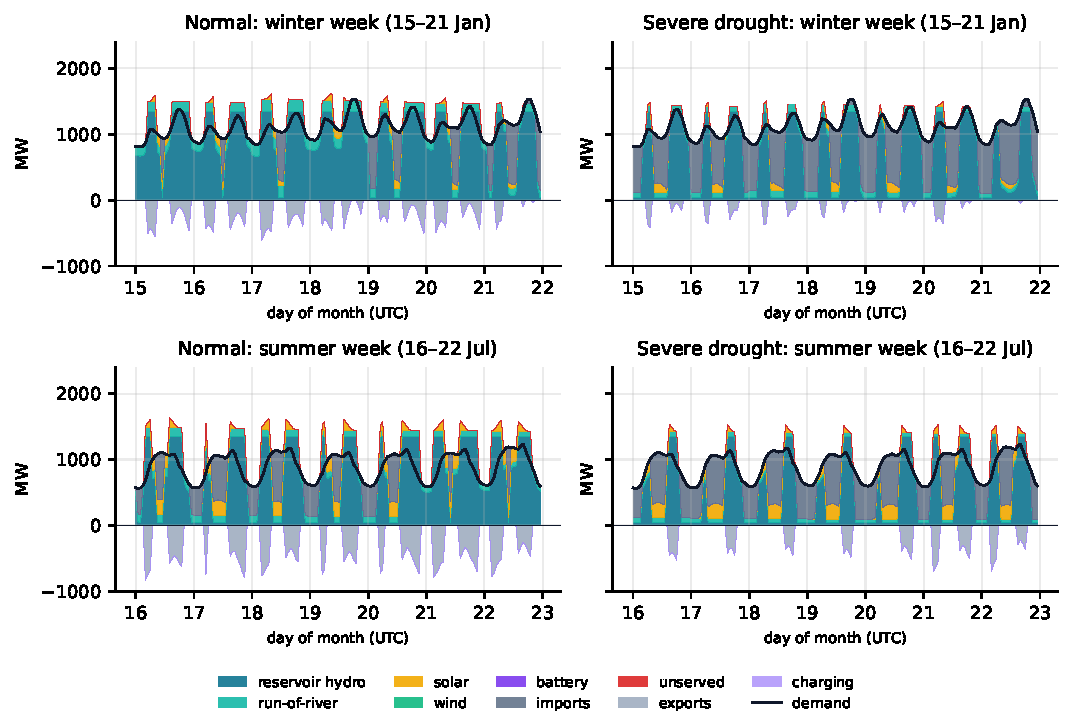
\includegraphics[width=\textwidth]{fig04_dispatch_normal_vs_drought.pdf}
\caption{Hourly dispatch in a winter and a summer week under normal conditions and severe drought (existing
fleet, full-year optimisation). Exports and battery charging are drawn below zero. In drought the reservoir
covers fewer hours and imports fill the evening peaks.}
\label{fig:dispatch}
\end{figure}

\begin{figure}[htbp]
\centering
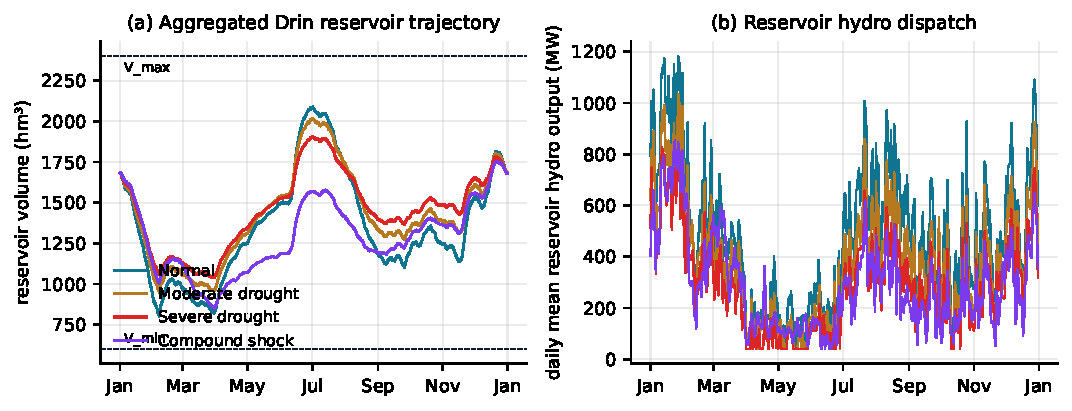
\includegraphics[width=\textwidth]{fig05_reservoir.pdf}
\caption{(a) Volume trajectory of the aggregated Drin reservoir and (b) daily reservoir hydro output under the
four presets (full-year hourly optimisation with $V_T=V_0$). The minimum operating volume is not reached in any
preset. Drought lowers releases rather than draining the reservoir, because the cyclic terminal condition
forces the deficit to be covered by imports.}
\label{fig:reservoir}
\end{figure}

\begin{table}[htbp]
\centering
\footnotesize
\caption{Annual hourly dispatch (8760 h, reference weather year). Energies in TWh, ENS in MWh, operating cost (imports $-$ exports + penalties + variable O\&M) in MEUR/yr, mean shadow price in EUR/MWh. Existing fleet unless stated.}
\label{tab:annual}
\begin{adjustbox}{max width=\linewidth}
\begin{tabular}{lrrrrrrrr}
\toprule
Case & Demand & Hydro & PV+wind & Imports & Exports & ENS & Opex & Price \\
\midrule
Normal & 8.00 & 6.77 & 0.46 & 2.00 & 1.23 & 0 & 40.8 & 97.2 \\
Moderate drought & 8.00 & 5.28 & 0.46 & 2.91 & 0.66 & 0 & 192.7 & 99.9 \\
Severe drought & 8.00 & 4.06 & 0.46 & 3.79 & 0.32 & 0 & 324.5 & 102.2 \\
Compound shock & 8.64 & 4.06 & 0.46 & 4.20 & 0.09 & 0 & 727.1 & 209.3 \\
Coordinated fleet, normal & 8.00 & 6.77 & 2.28 & 1.22 & 2.20 & 0 & -133.1 & 93.5 \\
Coordinated fleet, severe & 8.00 & 4.06 & 2.28 & 2.63 & 0.90 & 0 & 139.4 & 99.4 \\
\bottomrule
\end{tabular}
\end{adjustbox}
\end{table}


\subsection{Where reliability fails: interconnector availability and demand growth (Experiments F, G)}
A uniform import-price shock leaves dispatch unchanged, because relative prices stay the same. Annual cost
then rises linearly, from 324.5~MEUR at 1$\times$ to 968.4~MEUR at 3$\times$ (severe drought), with zero
unserved energy (Table~\ref{tab:exp-F}). Shortage appears only when import \emph{availability} falls. Under
severe drought with 8\% demand growth, availability of 75\% still serves all demand. At 50\%, 311~GWh are
unserved over 999~h with a peak shortfall of 811~MW. At 35\% and 25\% availability, unserved energy rises
to 1.40 and 2.16~TWh. These shortages are \emph{energy}-limited, not power-limited. With 50\% availability the
annual supply that can be delivered (hydro + PV + 450~MW of imports $\times$ 8{,}760~h) falls short of demand.
Consistent with this, a 400~MW / 1{,}600~MWh battery reduces unserved energy at 50\% availability by only 13\%
(311 to 270~GWh). At VOLL = 5{,}000~EUR/MWh even this partial reduction lowers annual cost by 199.8~MEUR,
well above the battery's 51.7~MEUR/yr annualised cost. At 35\% and 25\% availability the reduction is
1--2\% and the saving 97 and 59~MEUR/yr. Demand growth shows the same threshold behaviour (Table~\ref{tab:exp-G},
Fig.~\ref{fig:imports}c). With full interconnector availability, demand growth of up to 30\% is absorbed by
imports. With 50\% availability, unserved energy is 0, 456, 1{,}201 and 1{,}969~GWh at growth of 0, 10, 20 and
30\%, so loss-of-load hours rise from 0 to 4{,}088. In this model, therefore, the reliability of a
hydro-dependent system in drought is governed mainly by the availability of interconnection. This matters
because regional droughts can depress neighbours' export capacity at the same time.

\begin{table}[htbp]
\centering
\footnotesize
\caption{Experiment F: import price shocks and interconnector derating under severe drought (annual, hourly).}
\label{tab:exp-F}
\begin{tabular}{lrrrrr}
\toprule
Case (severe drought) & Imports (TWh) & Net imp. (TWh) & LOLH (h) & ENS (MWh) & Cost (MEUR/yr) \\
\midrule
Import price ×1.0 & 3.79 & 3.48 & 0 & 0 & 324.5 \\
Import price ×1.5 & 3.79 & 3.48 & 0 & 0 & 485.5 \\
Import price ×2.0 & 3.79 & 3.48 & 0 & 0 & 646.5 \\
Import price ×2.5 & 3.79 & 3.48 & 0 & 0 & 807.4 \\
Import price ×3.0 & 3.79 & 3.48 & 0 & 0 & 968.4 \\
NTC avail. 100%, +8\% demand & 4.33 & 4.12 & 0 & 0 & 391.7 \\
NTC avail. 75%, +8\% demand & 4.24 & 4.12 & 0 & 0 & 400.7 \\
NTC avail. 50%, +8\% demand & 3.81 & 3.81 & 999 & 310\,714 & 1\,957.2 \\
NTC avail. 35%, +8\% demand & 2.71 & 2.71 & 3\,391 & 1\,401\,990 & 7\,298.1 \\
NTC avail. 25%, +8\% demand & 1.95 & 1.95 & 4\,310 & 2\,162\,994 & 11\,022.9 \\
NTC 50%, +8\% dem., battery 400/1600 & 3.86 & 3.86 & 816 & 270\,120 & 1\,757.4 \\
NTC 35%, +8\% dem., battery 400/1600 & 2.74 & 2.74 & 3\,293 & 1\,382\,198 & 7\,200.9 \\
NTC 25%, +8\% dem., battery 400/1600 & 1.97 & 1.97 & 4\,267 & 2\,151\,012 & 10\,964.1 \\
\bottomrule
\end{tabular}
\end{table}


\subsection{Solar, storage and coordination (Experiments C, D, E)}
\paragraph{Solar without storage.} Adding PV reduces gross imports with diminishing returns
(Table~\ref{tab:exp-C}). Under normal conditions the reduction per added MW is 1{,}074, 898 and 699~MWh/MW
for +500, +1{,}000 and +1{,}500~MW. Under severe drought it is larger (1{,}406, 1{,}253 and 1{,}022~MWh/MW),
because a drier system exports less and imports more at the margin. Operating savings fall only slightly per
MW (138 to 131~kEUR/MW-yr in the normal year), because surplus midday PV can still be exported at 85\% of the
import price. Curtailment therefore stays small: at most 21~GWh, at +1{,}500~MW in the normal year. This
result rests on the assumed export capacity and price ratio (Section~\ref{sec:sensitivity}). The annualised
cost of PV is 80~kEUR/MW-yr, so under these assumptions every tested PV addition reduces total cost.

\paragraph{Batteries without new renewables.} A battery earns only intra-day arbitrage. The annual operating
savings are 5.5, 9.8 and 13.8~MEUR (normal) and 7.0, 12.7 and 17.9~MEUR (severe drought) for
200/800, 400/1{,}600 and 800/3{,}200~MW/MWh. Their annualised costs are 25.8, 51.7 and 103.3~MEUR/yr, so
arbitrage alone does not recover them. The value per unit is higher in drought, because the import price, not
the cheap reservoir, sets the marginal cost in more hours. Batteries also \emph{increase} gross imports: by
0.23--0.60~TWh in the normal year and similar amounts in the severe-drought year. They do this by storing
low-price imports for high-price hours. ``Reducing imports'' and ``reducing cost'' are therefore different
objectives for storage.

\paragraph{Coordination.} Combining PV (+1{,}000~MW) with a 400~MW / 1{,}600~MWh battery saves 146.9~MEUR/yr
in the normal year. That is 1.75~MEUR more than the sum of the separate savings (135.4 + 9.8). In severe
drought the corresponding synergy is 1.82~MEUR (Table~\ref{tab:exp-E}). The synergy is positive but small,
because an export route and the reservoir already absorb most PV surplus. The battery removes the remaining
2.2~GWh of PV curtailment.

\IfFileExists{tables/tab_exp_C.tex}{\begin{table}[htbp]
\centering
\footnotesize
\caption{Experiment C: PV additions without storage (annual, hourly).}
\label{tab:exp-C}
\begin{tabular}{lrrrrrr}
\toprule
Case & Imports (TWh) & Net imp. (TWh) & Curtail. (GWh) & Batt. cycles & ENS (MWh) & Opex (MEUR/yr) \\
\midrule
Normal, PV 300 MW & 2.00 & 0.77 & 0.0 & 0.0 & 0 & 40.8 \\
Normal, PV 800 MW & 1.46 & 0.00 & 0.0 & 0.0 & 0 & -28.3 \\
Normal, PV 1300 MW & 1.10 & -0.76 & 2.2 & 0.0 & 0 & -94.6 \\
Normal, PV 1800 MW & 0.95 & -1.51 & 20.7 & 0.0 & 0 & -156.3 \\
Severe, PV 300 MW & 3.79 & 3.48 & 0.0 & 0.0 & 0 & 324.5 \\
Severe, PV 800 MW & 3.09 & 2.71 & 0.0 & 0.0 & 0 & 252.7 \\
Severe, PV 1300 MW & 2.54 & 1.94 & 0.0 & 0.0 & 0 & 182.8 \\
Severe, PV 1800 MW & 2.26 & 1.18 & 2.3 & 0.0 & 0 & 117.0 \\
\bottomrule
\end{tabular}
\end{table}
}{}
\IfFileExists{tables/tab_exp_E.tex}{\begin{table}[htbp]
\centering
\footnotesize
\caption{Experiment E: coordinated portfolios (fixed fleets, annual hourly dispatch). Battery = 400 MW / 1600 MWh.}
\label{tab:exp-E}
\begin{adjustbox}{max width=\linewidth}
\begin{tabular}{lrrrrrr}
\toprule
Case & Imports (TWh) & Net imp. (TWh) & Curtail. (GWh) & Batt. cycles & ENS (MWh) & Opex (MEUR/yr) \\
\midrule
Normal, baseline & 2.00 & 0.77 & 0.0 & 0.0 & 0 & 40.8 \\
Normal, pv+1000 & 1.10 & -0.76 & 2.2 & 0.0 & 0 & -94.6 \\
Normal, batt400/1600 & 2.42 & 0.84 & 0.0 & 401.4 & 0 & 31.0 \\
Normal, pv+1000\&batt & 1.35 & -0.70 & 0.0 & 390.0 & 0 & -106.2 \\
Normal, pv+1000\&wind300 & 0.99 & -1.05 & 2.8 & 0.0 & 0 & -121.7 \\
Normal, pv+1000\&wind300\&batt & 1.22 & -0.99 & 0.0 & 385.1 & 0 & -133.1 \\
Severe, baseline & 3.79 & 3.48 & 0.0 & 0.0 & 0 & 324.5 \\
Severe, pv+1000 & 2.54 & 1.94 & 0.0 & 0.0 & 0 & 182.8 \\
Severe, batt400/1600 & 4.20 & 3.56 & 0.0 & 463.8 & 0 & 311.8 \\
Severe, pv+1000\&batt & 2.84 & 2.02 & 0.0 & 470.3 & 0 & 168.3 \\
Severe, pv+1000\&wind300 & 2.34 & 1.66 & 0.0 & 0.0 & 0 & 153.8 \\
Severe, pv+1000\&wind300\&batt & 2.63 & 1.74 & 0.0 & 468.5 & 0 & 139.4 \\
\bottomrule
\end{tabular}
\end{adjustbox}
\end{table}
}{}

\begin{figure}[htbp]
\centering
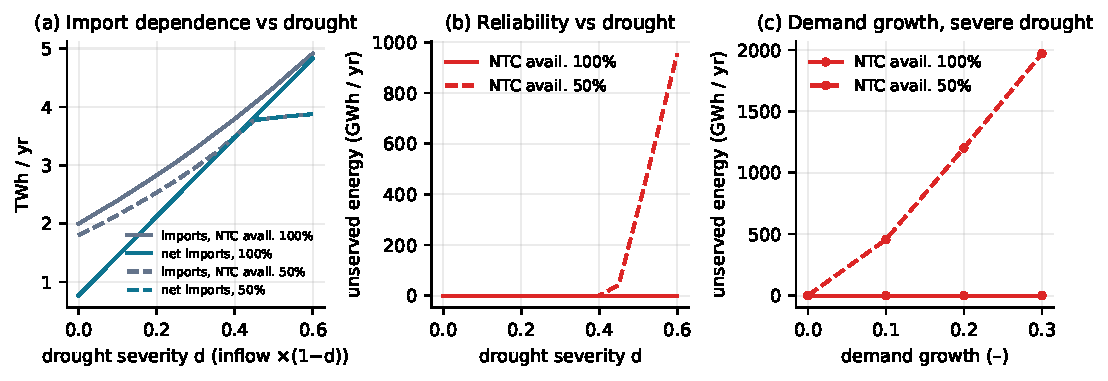
\includegraphics[width=\textwidth]{fig07_imports_reliability.pdf}
\caption{(a) Gross and net imports and (b) unserved energy as functions of drought severity $d$ (inflows scaled by
$1-d$, existing fleet) with full (solid) and halved (dashed) interconnector availability. (c) Unserved energy
under severe drought as demand grows. Shortage appears only when transfer availability is restricted.}
\label{fig:imports}
\end{figure}

\begin{figure}[htbp]
\centering
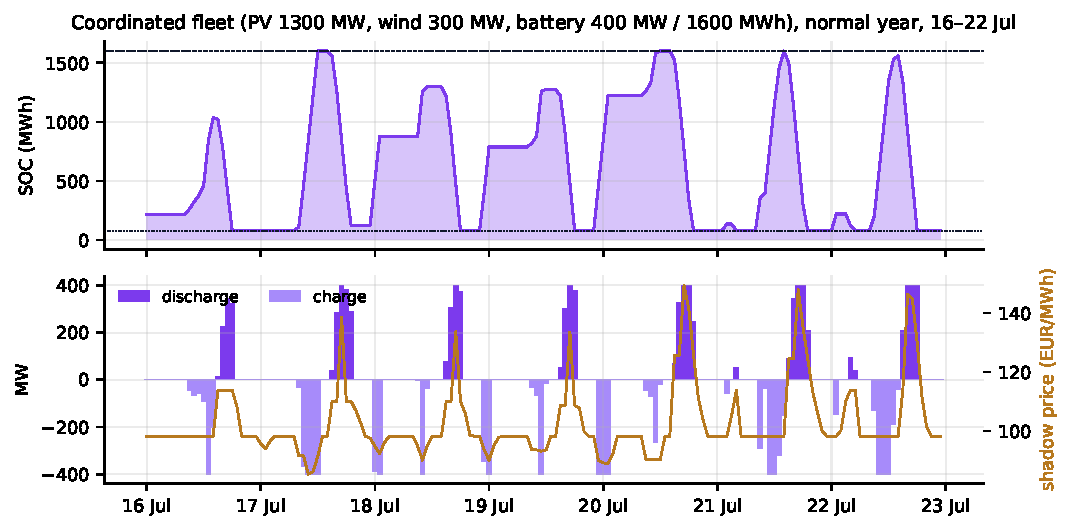
\includegraphics[width=\textwidth]{fig06_battery_soc.pdf}
\caption{Battery operation in a summer week (coordinated fleet: PV 1{,}300~MW, wind 300~MW, battery 400~MW /
1{,}600~MWh). The battery charges around midday when PV depresses the shadow price and discharges in the
evening peak: roughly one cycle per day (385 equivalent full cycles per year).}
\label{fig:battery}
\end{figure}

\subsection{Marginal value of flexibility (Experiment J)}
Table~\ref{tab:marginal} and Fig.~\ref{fig:marginal} report finite-difference and dual-based marginal values
around a base fleet with PV 300~MW, a 200~MW / 800~MWh battery and 900~MW of import capacity. In every
non-degenerate case the dual lies within the finite-difference interval $[\Delta^+,\Delta^-]$, as LP theory
predicts. Four results stand out:
\begin{itemize}
\item \textbf{PV} has an operating value of 140~kEUR/MW-yr (normal), 146 (severe drought) and 314 (compound
shock), against an annualised cost of 80~kEUR/MW-yr.
\item \textbf{Wind} (CF $\approx$ 0.11 from coarse reanalysis) is worth 93--99~kEUR/MW-yr against 133~kEUR/MW-yr
in normal and drought years, and 202 under the compound shock. The wind dual at zero capacity is flagged as a
degenerate corner, and the right finite difference is reported instead.
\item \textbf{Battery power and energy are not substitutes.} With 800~MWh installed, an extra MW of discharge
power is worth 12.7--15.5~kEUR/yr in normal and drought years, above its 10.1~kEUR/yr annualised cost.
An extra MWh is worth only 2.3--4.1~kEUR/yr, against 29.8. Shorter-duration batteries are therefore closer
to break-even than the 4-hour configuration.
\item \textbf{Import capacity} is worth 2~kEUR/MW-yr in a normal year, 9 in severe drought and 175 under the
compound shock. This is the largest increase of any resource, and it confirms that interconnection is the
critical flexibility resource under compound stress. Additional reservoir \emph{volume} has zero marginal value
in all cases: the volume bound never binds, and the energy limit comes from inflow rather than storage size.
\end{itemize}

\begin{table}[htbp]
\centering
\footnotesize
\caption{Marginal operating value of flexibility (kEUR per unit per year) around the base fleet (PV 300 MW, battery 200 MW/800 MWh, NTC 900 MW, $V^{\max}$ 2400 hm$^3$). $\Delta^+$: value of adding the next increment; $\Delta^-$: value of the last increment. Ann. cost: annualised cost of one more unit.}
\label{tab:marginal}
\begin{adjustbox}{max width=\linewidth}
\begin{tabular}{lrrrrrrr}
\toprule
Resource & Scenario & Unit & $\Delta^+$ & $\Delta^-$ & Dual & Dual valid & Ann. cost \\
\midrule
battery energy & normal & MWh & 2.3 & 3.0 & 2.6 & yes & 29.8 \\
battery power & normal & MW & 12.7 & 16.2 & 14.5 & yes & 10.1 \\
solar pv & normal & MW & 139.7 & 140.0 & 139.8 & yes & 80.1 \\
wind & normal & MW & 92.8 & -- & 92.9 & no & 132.7 \\
import capacity & normal & MW & 1.7 & 2.7 & 2.1 & yes & 30.0 \\
reservoir volume & normal & hm$^3$ & 0.0 & 0.0 & 0.0 & yes & -- \\
battery energy & severe drought & MWh & 3.1 & 4.1 & 3.3 & yes & 29.8 \\
battery power & severe drought & MW & 15.5 & 20.3 & 18.6 & yes & 10.1 \\
solar pv & severe drought & MW & 145.6 & 146.1 & 145.8 & yes & 80.1 \\
wind & severe drought & MW & 99.2 & -- & 99.3 & no & 132.7 \\
import capacity & severe drought & MW & 7.5 & 11.2 & 9.3 & yes & 30.0 \\
reservoir volume & severe drought & hm$^3$ & 0.0 & 0.0 & 0.0 & yes & -- \\
battery energy & compound shock & MWh & 4.1 & 5.4 & 4.6 & yes & 29.8 \\
battery power & compound shock & MW & 8.2 & 11.7 & 10.0 & yes & 10.1 \\
solar pv & compound shock & MW & 314.2 & 322.1 & 318.1 & yes & 80.1 \\
wind & compound shock & MW & 201.8 & -- & 202.5 & no & 132.7 \\
import capacity & compound shock & MW & 153.5 & 197.4 & 174.5 & yes & 30.0 \\
reservoir volume & compound shock & hm$^3$ & 0.0 & 0.0 & 0.0 & yes & -- \\
\bottomrule
\end{tabular}
\end{adjustbox}
\end{table}


\begin{figure}[htbp]
\centering
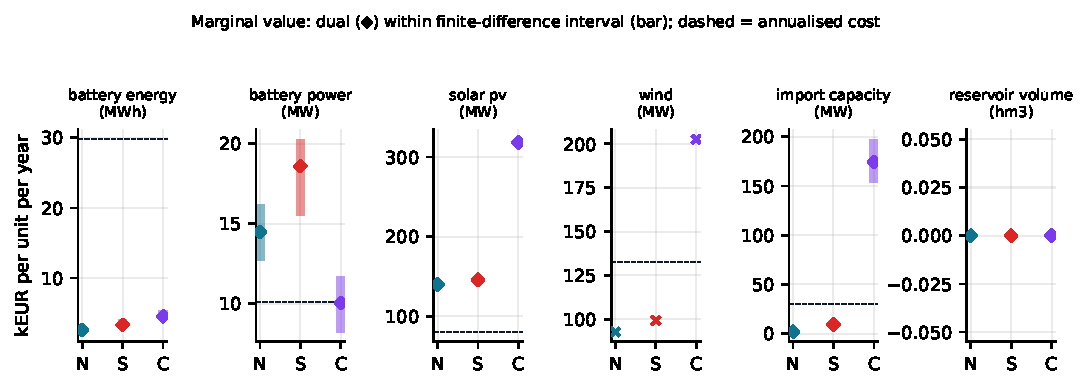
\includegraphics[width=\textwidth]{fig11_marginal_value.pdf}
\caption{Marginal operating value of each flexibility resource in the normal (N), severe-drought (S) and
compound-shock (C) cases. Bars show the finite-difference interval $[\Delta^+,\Delta^-]$, diamonds the dual
value (crosses mark degenerate corners), and the dashed line the annualised cost of one more unit.}
\label{fig:marginal}
\end{figure}

\subsection{Budget-constrained investment (Experiment H)}
For the normal year, the deterministic optimum spends every budget level from 100 to 1{,}500~MEUR entirely on
PV: 126, 315, 629, 944, 1{,}258 and 1{,}888~MW. At 2{,}000~MEUR the PV bound (+2{,}000~MW) binds and the
budget does not. Neither wind nor storage enters at any budget. The budget shadow price falls from 0.070 to
0.024~EUR of annual saving per euro of capital as PV grows. These are diminishing but still positive returns,
and they are consistent with the PV marginal value of Experiment~J (140~kEUR/MW-yr against 80~kEUR/MW-yr of
annualised cost). The result reflects three assumptions: exports absorb midday surplus at 85\% of the import
price, there is no reserve requirement, and wind capacity factors are about 0.11 from coarse reanalysis.
Section~\ref{sec:sensitivity} tests the first of these.

\subsection{Deterministic versus stochastic planning (Experiment I)}
The two-stage programme has five scenarios, eight hourly weeks each, a 500~MEUR budget and CVaR at $\alpha=0.9$.
For every risk weight tested ($\lambda\in\{0,0.25,1,4\}$) it selects the \emph{same} portfolio as the
deterministic normal-year plan: +629~MW of PV, with no wind and no storage (Table~\ref{tab:risk-sweep}). The same
holds at a 1{,}500~MEUR budget. Each wait-and-see problem also chooses this plan, so the value of the stochastic
solution and the expected value of perfect information are both zero to solver precision
(Table~\ref{tab:stochastic}). CVaR$_{0.9}$ of operating cost is 397~MEUR/yr for both plans. Hypothesis~I is
therefore \textbf{not supported} under the base assumptions. PV is a \emph{no-regret} investment in every
scenario. Its value is set mainly by the import price, and it rises under stress. The budget binds before any
resource whose value depends on the scenario becomes competitive. The stochastic machinery still answers
question~6 of the study: under these assumptions, deterministic planning for an average year is not
penalised. One qualification matters. None of the five planning scenarios, the compound shock included
(70\% availability), reaches the import-availability regime of $\le$50\% in which shortages occur and
batteries become valuable (Sections~\ref{sec:results} and~\ref{sec:sensitivity}). A scenario set with even a
small probability of that regime could change the plan, and this is a priority for future work.

\IfFileExists{tables/tab_stochastic.tex}{\begin{table}[htbp]
\centering
\small
\caption{Two-stage stochastic versus deterministic planning (budget 500 MEUR, 8 representative weeks, water-value boundaries). E[cost]: expected total annualised cost (MEUR/yr) on all five scenarios; CVaR of operating cost (MEUR/yr). Risk-adjusted VSS = 0.00 MEUR/yr; EVPI is reported only for $\lambda=0$.}
\label{tab:stochastic}
\begin{adjustbox}{max width=\linewidth}
\begin{tabular}{lrrrrrr}
\toprule
Plan & +PV & +Wind & +B MW & +B MWh & E[cost] & CVaR$_{0.9}$ \\
\midrule
Stochastic (RP), $\lambda$=1 & 629 & 0 & 0 & 0 & 70.9 & 397.3 \\
Deterministic (normal year) & 629 & 0 & 0 & 0 & 70.9 & 397.3 \\
\bottomrule
\end{tabular}
\end{adjustbox}
\end{table}
}{}

\subsection{When does stochastic planning matter? (Experiment I2)}
To find the conditions under which uncertainty changes the decision, we repeated the comparison with export
capacity limited to 300~MW. Surplus PV must then be stored, absorbed by the reservoir or curtailed. We also
raised the budget, so that PV saturates before the budget binds (Table~\ref{tab:i2}). With 900~MW of export
capacity the stochastic and deterministic plans remain identical at every risk weight (VSS = 0). With
restricted exports and risk-neutral planning ($\lambda=0$), the stochastic plan adds slightly more PV than the
deterministic one (+26~MW at 1{,}000~MEUR, +75~MW at 1{,}500~MEUR), and the VSS is only 0.2--0.3~MEUR/yr. With
restricted exports, a 1{,}500~MEUR budget and $\lambda=1$, the decision changes qualitatively. The risk-averse
plan adds 1{,}520~MW of PV, 230~MW of \emph{wind} and a 30~MW / 66~MWh battery. The deterministic plan adds
1{,}232~MW of PV only. In the representative-week model the risk-averse plan raises expected cost by
7.8~MEUR/yr and lowers CVaR$_{0.9}$ of operating cost by 79~MEUR/yr (from 292 to 213); the risk-adjusted VSS is
71.5~MEUR/yr. Full-year chronological re-evaluation of the two plans confirms the trade-off. Expected total
cost is higher by 15.1~MEUR/yr (74.6 vs 59.5), CVaR$_{0.9}$ of operating cost is lower by 74.5~MEUR/yr (208.2
vs 282.7), and neither plan has any unserved energy. The hedge is mainly wind rather than storage. Once PV saturates
under the export limit, wind is the cheapest remaining way to cut imports in the high-price stress scenarios.
We did not decompose this mechanism further, for example by wind--PV correlation or season. Stochastic, risk-aware planning therefore matters when a no-regret resource
saturates because its surplus cannot leave the system. In that regime the choice among the remaining resources
depends on the tail scenarios.

\IfFileExists{tables/tab_i2.tex}{\input{tables/tab_i2}}{}

\begin{figure}[htbp]
\centering
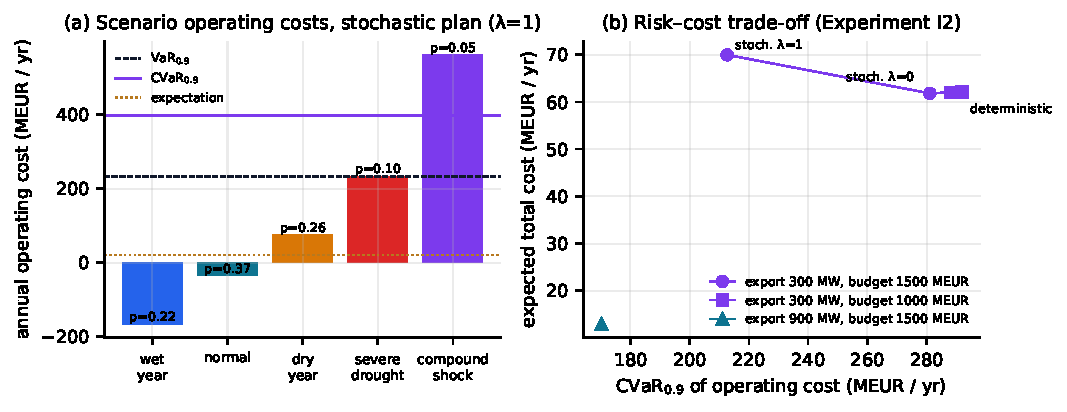
\includegraphics[width=\textwidth]{fig09_cvar.pdf}
\caption{(a) Annualised operating cost of the reference stochastic plan in each scenario, with probabilities, VaR$_{0.9}$,
CVaR$_{0.9}$ and the expectation. In the base case this plan is identical to the deterministic plan. (b) Expected total cost
versus CVaR$_{0.9}$ of operating cost for the deterministic plan and the stochastic plans ($\lambda=0,1$) in
Experiment~I2. Only with restricted exports and a large budget does risk aversion buy a material reduction in tail
cost.}
\label{fig:cvar}
\end{figure}


\subsection{Investment frontier}
Figure~\ref{fig:frontier} and Table~\ref{tab:strategies} compare the required strategies, the budget sweep and
the stochastic plans on equal terms, using the same representative-week evaluation. At 500~MEUR the strategies
rank as follows by expected total annualised cost: solar (70.9~MEUR/yr; identical to the coordinated and
climate-robust optima), baseline (109.4), wind (112.1) and battery-only (164.9). The battery-only plan has the
highest cost and the highest imports, because arbitrage increases gross imports. Across budgets, larger PV
additions lower both expected cost and imports. The non-dominated set in (expected cost, expected imports)
therefore collapses to the largest-PV plan, and the trade-off appears only in capital spent versus imports
(\texttt{pareto\_capex\_imports} in the artefact). We report this degenerate frontier as it is, rather than
constructing an artificial trade-off.

\begin{figure}[htbp]
\centering
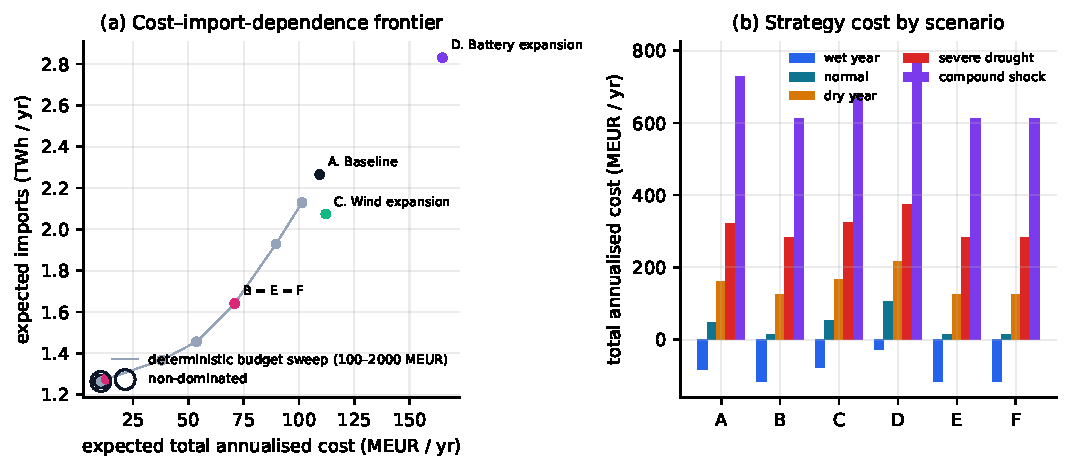
\includegraphics[width=\textwidth]{fig08_investment_frontier.pdf}
\caption{(a) Strategies in the plane of expected total annualised cost and expected imports, evaluated with the
same representative-week model over five scenarios. Outlined points are non-dominated. (b) Total annualised cost
of the required strategies A--F in each scenario.}
\label{fig:frontier}
\end{figure}

\begin{table}[htbp]
\centering
\scriptsize
\caption{Investment strategies evaluated on the five-scenario set (representative weeks, hourly). Additions in MW/MWh, overnight capex in MEUR, expected total annualised cost and severe-drought cost in MEUR/yr, expected imports in TWh/yr; ND marks the non-dominated set in (expected cost, expected imports).}
\label{tab:strategies}
\begin{tabular}{p{4.2cm}rrrrrrrrc}
\toprule
Strategy & +PV & +Wind & +B MW & +B MWh & Capex & E[cost] & E[imp.] & Cost sev. & ND \\
\midrule
A. Baseline & 0 & 0 & 0 & 0 & 0 & 109.4 & 2.27 & 320.4 &  \\
B. Solar expansion & 629 & 0 & 0 & 0 & 500 & 70.9 & 1.64 & 283.5 &  \\
C. Wind expansion & 0 & 418 & 0 & 0 & 500 & 112.1 & 2.07 & 323.7 &  \\
D. Battery expansion & 0 & 0 & 522 & 2\,087 & 500 & 164.9 & 2.83 & 373.4 &  \\
E. Coordinated (deterministic optimum) & 629 & 0 & 0 & 0 & 500 & 70.9 & 1.64 & 283.5 &  \\
F. Climate-robust (stochastic, CVaR λ=1) & 629 & 0 & 0 & 0 & 500 & 70.9 & 1.64 & 283.5 &  \\
Budget 100 MEUR (det.) & 126 & 0 & 0 & 0 & 100 & 101.4 & 2.13 & 312.9 &  \\
Budget 250 MEUR (det.) & 315 & 0 & 0 & 0 & 250 & 89.7 & 1.93 & 301.8 &  \\
Budget 750 MEUR (det.) & 944 & 0 & 0 & 0 & 750 & 53.7 & 1.46 & 266.5 &  \\
Budget 1000 MEUR (det.) & 1\,258 & 0 & 0 & 0 & 1\,000 & 37.9 & 1.37 & 251.2 &  \\
Budget 1500 MEUR (det.) & 1\,888 & 0 & 0 & 0 & 1\,500 & 12.9 & 1.27 & 225.1 &  \\
Budget 2000 MEUR (det.) & 2\,000 & 0 & 0 & 0 & 1\,589 & 10.4 & 1.26 & 222.3 & $\bullet$ \\
Stochastic λ=0.0 (500 MEUR) & 629 & 0 & 0 & 0 & 500 & 70.9 & 1.64 & 283.5 &  \\
Stochastic λ=0.25 (500 MEUR) & 629 & 0 & 0 & 0 & 500 & 70.9 & 1.64 & 283.5 &  \\
Stochastic λ=4.0 (500 MEUR) & 629 & 0 & 0 & 0 & 500 & 70.9 & 1.64 & 283.5 &  \\
Stochastic λ=0.0 (1500 MEUR) & 1\,888 & 0 & 0 & 0 & 1\,500 & 12.9 & 1.27 & 225.1 &  \\
Stochastic λ=4.0 (1500 MEUR) & 1\,888 & 0 & 0 & 0 & 1\,500 & 12.9 & 1.27 & 225.1 &  \\
\bottomrule
\end{tabular}
\end{table}


\subsection{Validity of the representative-week approximation}
\label{sec:chrono}
Seven plans were re-evaluated with full-year chronological hourly dispatch on all five scenarios. With the
water-value boundary, the representative-week model's expected total cost differs from chronology by 1.7 to
10.0~MEUR/yr in absolute terms. It overstates the cost of the PV plans by 4.2--8.7~MEUR/yr and understates the
wind plan by 10.0~MEUR/yr. Both models find no unserved energy for any plan, and the strategies rank in the
same order (ties between identical plans aside). An earlier variant pinned each week's terminal volume
($V_T\ge\bar V^T$). That variant overstated cost by up to 20.4~MEUR/yr and produced spurious shortages in the
sampled drought weeks. Those shortages made a PV--battery portfolio look better on tail risk, but full
chronology showed this to be an artefact: the PV-only plan had lower expected cost (66.7 vs 76.3~MEUR/yr) and
lower CVaR (443.5 vs 455.7~MEUR/yr). We report this as a methodological finding. How the seasonal boundary of a
representative period is treated can change the investment recommendation, and validation against full
chronology should be routine.

\IfFileExists{tables/tab_chrono.tex}{\begin{table}[htbp]
\centering
\footnotesize
\caption{Full-year chronological (8760 h, hourly) versus representative-week (8 weeks, water-value boundaries) evaluation of the same plans on the five-scenario set. Costs in MEUR/yr; CVaR$_{0.9}$ of total annualised cost; ENS expected MWh/yr.}
\label{tab:chrono}
\begin{adjustbox}{max width=\linewidth}
\begin{tabular}{p{5cm}rrrrrr}
\toprule
Plan & E[cost] chrono & E[cost] rep. & Diff. & CVaR chrono & CVaR rep. & ENS chrono \\
\midrule
A. Baseline & 107.7 & 109.4 & 1.7 & 525.8 & 524.0 & 0 \\
B. Solar expansion & 66.7 & 70.9 & 4.2 & 443.5 & 447.7 & 0 \\
C. Wind expansion & 122.1 & 112.1 & -10.0 & 520.0 & 502.9 & 0 \\
D. Battery expansion & 162.8 & 164.9 & 2.1 & 577.9 & 576.9 & 0 \\
F. Climate-robust (stochastic, CVaR λ=1) & 66.7 & 70.9 & 4.2 & 443.5 & 447.7 & 0 \\
Budget 1500 MEUR (det.) & 4.2 & 12.9 & 8.7 & 308.6 & 321.4 & 0 \\
Stochastic λ=0.0 (500 MEUR) & 66.7 & 70.9 & 4.2 & 443.5 & 447.7 & 0 \\
\bottomrule
\end{tabular}
\end{adjustbox}
\end{table}
}{}


\section{Sensitivity and robustness}
\label{sec:sensitivity}

\paragraph{Tornado analysis of the investment decision.} For each of nine parameters we re-optimised the
normal-year investment problem (500~MEUR, representative weeks) at a low and a high value
(Fig.~\ref{fig:sensitivity}a). The optimal annualised system cost is most sensitive to the following
parameters, in decreasing order of effect:
\begin{itemize}
\item drought severity: $+213.5$~MEUR/yr at $d=0.3$;
\item demand ($\pm10\%$): $-74.3$/$+68.4$~MEUR/yr;
\item the export/import price ratio: $+30.0$/$-18.8$~MEUR/yr at 0.75/0.95;
\item PV capex ($\pm30\%$): $-34.7$/$+19.1$~MEUR/yr;
\item the import price ($\pm30\%$): $+13.3$/$-13.3$~MEUR/yr;
\item the discount rate (4\%/10\%): $-10.9$/$+12.1$~MEUR/yr.
\end{itemize}
The \emph{technology choice}, all PV, is unchanged across every case. Only the PV amount responds, to its own
capex: 899~MW at $\times0.7$ and 484~MW at $\times1.3$. The budget binds in both cases. VOLL and battery capex
have no effect because no shortage occurs and no battery is chosen. Interconnector capacity between 600 and
1{,}200~MW moves cost by less than 3~MEUR/yr in a normal year. The importance of interconnection appears only
under joint stress (Experiments F, G and J).

\paragraph{Drought severity sweep.} Increasing the inflow reduction $d$ from 0 to 0.6 in steps of 0.05, with
the existing fleet, raises imports almost linearly: from 2.0 to 4.9~TWh/yr with full transfer availability,
while annual cost rises from 41 to 481~MEUR (Fig.~\ref{fig:imports}a). No shortage occurs at any severity with
full availability. With 50\% availability the system copes up to $d=0.4$, and unserved energy then jumps to
341~GWh at $d=0.5$ and 956~GWh at $d=0.6$ (Fig.~\ref{fig:imports}b). The reliability boundary of the system
therefore lies in the joint space of drought severity and import availability.

\paragraph{Battery value across drought and import stress.} With import availability at 60\%, the net benefit
of a 4-hour battery (operating saving minus annualised cost) is negative up to drought severity $d=0.4$:
between $-10$ and $-97$~MEUR/yr for 400--3{,}200~MWh (Fig.~\ref{fig:sensitivity}b). It turns strongly positive
at $d=0.6$, where shortage occurs: $+248$ to $+332$~MEUR/yr. There the battery reduces unserved energy from 281
to between 228 and 192~GWh, and each avoided MWh is valued at VOLL. Batteries in this system are therefore
\emph{reliability} assets under joint drought and import stress, not arbitrage assets. Their economic case
depends on the probability of such joint events and on the VOLL assumed for them. This is the case where
the VOLL assumption matters most.

\paragraph{Temporal resolution.} The operating saving from a 400~MW / 1{,}600~MWh battery is 9.8, 8.8, 7.0 and
1.3~MEUR/yr at 1-, 2-, 3- and 6-hour time steps, and its cycling falls from 401 to 111 equivalent full cycles
(Fig.~\ref{fig:resolution}). Six-hourly steps remove 87\% of the battery's arbitrage value. This explains why the
first, 6-hourly version of our stochastic model selected no storage, and why the investment studies use hourly
representative weeks.

\begin{figure}[htbp]
\centering
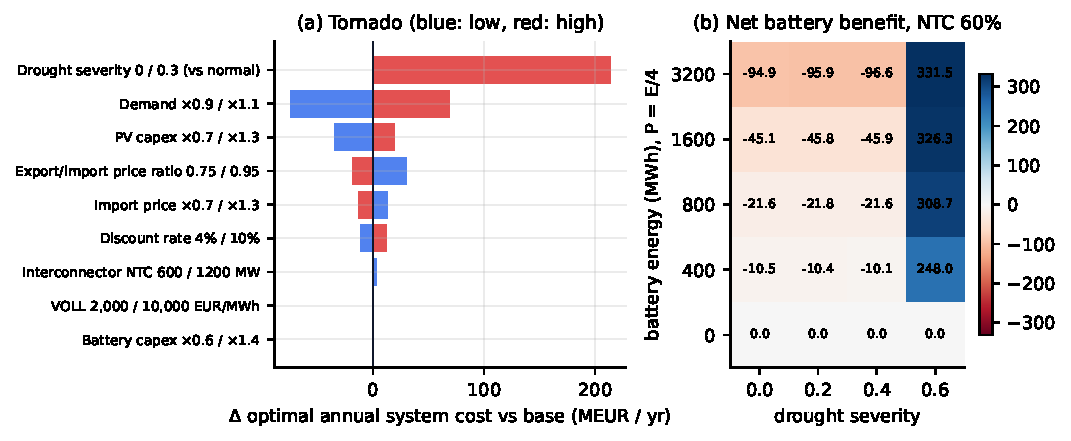
\includegraphics[width=\textwidth]{fig10_sensitivity.pdf}
\caption{(a) Change in the optimal annualised system cost when each parameter is set to its low (blue) or high
(red) value, with investment re-optimised each time. (b) Net annual benefit (MEUR/yr) of a 4-hour battery as a
function of drought severity and battery size, with import availability 60\%.}
\label{fig:sensitivity}
\end{figure}

\begin{figure}[htbp]
\centering
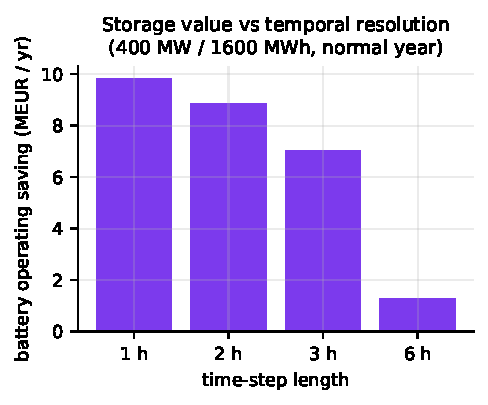
\includegraphics[width=0.5\textwidth]{fig12_resolution.pdf}
\caption{Operating value of a 400~MW / 1{,}600~MWh battery in the normal year as a function of the time-step
length.}
\label{fig:resolution}
\end{figure}

\section{Discussion}
\label{sec:discussion}

\paragraph{Drought as financial risk, interconnection as reliability risk.} The clearest result is a separation
of risks. With the interconnector available, even a 40\% inflow reduction is met entirely by imports. The cost
of drought is financial: operating cost rises by 284~MEUR/yr between the normal and the severe-drought year.
Unserved energy appears only when transfer availability falls to about half, and it is energy-limited.
Short-duration storage can therefore reduce it only partially (13\% at 50\% availability). At an assumed VOLL of
5{,}000~EUR/MWh, however, even that partial reduction is worth more than the battery costs. Batteries thus
earn their keep here as reliability assets in joint stress events, not as arbitrageurs. This agrees with the concern of van Vliet et
al.~\cite{vanvliet2016vulnerability} that climate impacts on water-dependent generation are partly
compensated by trade and partly transmitted to neighbours. It also suggests that, for Albania, the joint
probability of domestic drought and reduced regional export capacity deserves more attention than domestic
drought alone. Because Balkan hydro systems share weather, this joint risk is plausible. Our scenario
probabilities for it are assumed, not estimated.

\paragraph{Solar as a no-regret option, conditional on export.} Under the base assumptions, PV is worth about
1.7$\times$ its annualised cost at the margin. It dominates all other investments at every budget and in every
scenario, which is why VSS is zero. Two mechanisms drive this. First, in a reservoir system PV saves water,
which the reservoir then moves to high-price hours, so PV inherits part of the reservoir's flexibility value.
Second, surplus PV can be exported at 85\% of the import price. The decline of renewable market value with
penetration described by Hirth~\cite{hirth2013market} is therefore weak here, but only because the export
route is assumed to absorb the surplus. When exports are restricted (Experiment~I2), this conclusion changes.
That restriction is the condition under which planning for uncertainty starts to matter.

\paragraph{Storage: timing, not volume.} Batteries reduce cost by shifting energy in time. In doing so they
\emph{increase} gross imports, by importing cheaply and serving the evening peak. Policy goals stated as
``reducing import dependence'' and ``reducing system cost'' can therefore point in different directions for
storage. Arbitrage alone does not recover battery costs here: savings are 13--27\% of annualised cost across the tested sizes and years. The
economic case for batteries rests instead on avoided shortage in joint drought and import-stress events
(Section~\ref{sec:sensitivity}), and so on how likely those events are and what VOLL is assumed.
The marginal analysis shows, however, that discharge power is worth more than its cost once some energy
capacity exists. This points to shorter-duration systems and to the reserve and ancillary services that the
model omits \cite{lund2015flexibility,kondziella2016flexibility}. The reservoir already supplies long-duration
flexibility: additional reservoir \emph{volume} has zero marginal value in every case, because annual inflow,
not storage size, is the binding resource.

\paragraph{Methodological lessons.} Two modelling choices changed answers by more than many of the parameter
uncertainties. First, temporal resolution: at 6-hourly steps battery value nearly vanishes and stochastic
planning had nothing to choose between (Section~\ref{sec:sensitivity}), consistent with
Poncelet et al.~\cite{poncelet2016temporal}. Second, how the boundaries of representative periods are handled
for a seasonal store. Pinning each week's terminal volume created spurious scarcity. That made a battery look
valuable for tail risk and reversed the ranking of two plans compared with full chronology. Valuing the end
volume at the coarse annual run's water value, a single-cut future-cost function as in SDDP
\cite{pereira1991sddp}, removed the artefact. This is a concrete example of the seasonal-storage problem in
representative-period models described by Kotzur et al.~\cite{kotzur2018seasonal}. Our recommendation is that
studies of hydro-dominated systems validate their period selection against full chronology, as we do here.

\paragraph{Model implications versus policy.} These are implications of a single-node model with synthetic
demand and prices. They are not recommendations for Albanian policy. A credible policy analysis would need
observed hourly load (ENTSO-E), regional price and transfer-capacity data, calibrated hydrology and a network
representation. The open pipeline is designed so that each of these can be substituted without code changes
to the optimisation core.

\section{Limitations}
\label{sec:limitations}

\paragraph{Network representation.} The model has a single node. Internal transmission constraints, losses and
stability limits are absent. The four interconnections (Montenegro, Kosovo, North Macedonia, Greece) are
collapsed into one import and one export limit, so this is not a power-flow model. Regional correlation of
droughts and prices is represented only through the scenario availability factor $a_s$.

\paragraph{Market data.} Demand and prices are synthetic. Export revenue is a fixed 85\% of the import price.
Many conclusions, especially the value of PV, which in this model can always be exported up to 900~MW, depend
on this assumption. With observed ENTSO-E load and regional day-ahead prices the analysis could be repeated
without code changes.

\paragraph{Hydrology.} Inflows are reconstructed from reanalysis precipitation with an uncalibrated conceptual
model and scaled to an assumed mean energy. They are not gauged inflows. Drought is a uniform scaling of one
reference year. Real droughts also change the seasonal timing of inflows, and this is not captured.

\paragraph{Reservoir simplification.} The three-stage Drin cascade is one equivalent reservoir with a fixed
aggregate head. Head-dependent efficiency, travel times, individual reservoir limits and flood-control rules
are omitted. The other hydro plants are treated as run-of-river without storage.

\paragraph{Operational detail.} There is no unit commitment, no ramping, no reserve or ancillary-service
requirement and no thermal fleet. Batteries are therefore valued only for energy arbitrage and shortage
avoidance, which probably understates their real value. Simultaneous charging and discharging is excluded by
economics, not by binaries, and is monitored.

\paragraph{Time structure.} Investment and stochastic studies use eight representative weeks with
fleet-independent seasonal boundaries. Water allocation across seasons therefore does not adapt to new
investment. We quantify the error against full-year chronology (Section~\ref{sec:chrono}), but the planning
results inherit it.

\paragraph{Costs and uncertainty.} Technology costs are global IRENA averages with an assumed regional
multiplier. VOLL, the discount rate, lifetimes and the scenario probabilities are assumptions. Five scenarios
cannot describe the full climate distribution, and the 15\% stress probability is a judgement, not an estimate.

\paragraph{Validation.} The model has been \emph{verified}: against an independent PyPSA formulation and through
automated conservation and behaviour tests. It has \textbf{not been validated} against observed operations of
the Albanian system. Scenario comparisons are model experiments, not empirical evidence. The results are model
implications under stated assumptions and should not be read as policy recommendations.

\section{Conclusion}
\label{sec:conclusion}

We built and verified an open optimisation model of a hydropower-dependent electricity system. It couples
hourly dispatch, a physical reservoir water balance, batteries, imports and investment under uncertainty,
and it reports every result together with its data provenance and its limitations. Under the stated (partly
synthetic) assumptions, the experiments support the following defensible findings.
\begin{enumerate}
\item Drought is primarily a financial and import-dependence risk. Reliability is governed by the
availability of interconnection: shortages require import availability of about 50\% or less together with
severe drought or demand growth.
\item Solar PV is a no-regret investment in every scenario as long as its surplus can be exported. Its
marginal value is about 1.7$\times$ its annualised cost, and the technology choice is robust to every
sensitivity tested.
\item Batteries do not recover their cost through arbitrage, and they increase gross imports. They do pay
off through avoided unserved energy in joint drought and import-stress events. Discharge power is more
valuable than additional energy capacity.
\item Stochastic, CVaR-based planning changes the decision only when the dominant resource saturates. With
exports restricted, it buys a wind hedge that lowers tail cost by 74.5~MEUR/yr for 15.1~MEUR/yr of expected
cost, and this is confirmed by full chronology.
\item Methodologically, temporal resolution and the boundary treatment of representative periods for
seasonal storage each changed conclusions. Water-value boundaries and chronological validation are
inexpensive safeguards.
\end{enumerate}

\paragraph{Next steps.} (i)~Replace the synthetic demand and prices with observed ENTSO-E load and regional
market data. (ii)~Calibrate the hydrology against gauge or plant records and represent the three Drin stages
separately, with variable head. (iii)~Add network constraints for the four interconnections and correlated
regional scenarios, including the low-availability regime in which storage becomes valuable. (iv)~Add
reserve requirements and multi-stage hydro scheduling, for example SDDP-style water-value cuts. (v)~Estimate
scenario probabilities from climate-model ensembles rather than by assumption.


\section*{Data and code availability}
All code, input-data provenance records, experiment outputs and the scripts that generate every figure and
table in this manuscript are contained in the HYDROFLEX AI repository. Running
\texttt{python -m hydroflex.experiments.run_all} regenerates the experiment files, tables and figures.
Demand and price series are synthetic and are labelled as such in every output.

\section*{Use of software and AI assistance}
Model code, the experiment pipeline and draft text were developed with the assistance of an AI coding
assistant (Claude, Anthropic) operating under the author's direction. All reported numbers are produced by
executed code in the repository.

\bibliographystyle{unsrtnat}
\bibliography{references}

\appendix
\FloatBarrier
\section{Symbols}
\label{app:symbols}
\begin{table}[htbp]\centering\footnotesize
\caption{Symbols and units.}
\begin{tabular}{llp{9cm}}
\toprule
Symbol & Unit & Meaning \\
\midrule
$t,\ \Delta t,\ T$ & h & time step index, step length, number of steps \\
$s,\ \pi_s$ & -- & scenario and probability \\
$x_{pv},x_w$ & MW & installed PV and wind capacity (first stage) \\
$x_{bp},x_{be}$ & MW, MWh & battery power and energy capacity (first stage) \\
$x_{imp},\ x_{vmax}$ & MW, hm$^3$ & import capacity, maximum reservoir volume (fixed; marginal-value analysis) \\
$x^0_k,\ \bar x_k$ & & existing capacity, maximum addition \\
$A_k,\ C_k$ & kEUR/unit(-yr) & annualised and overnight cost \\
$w$ & -- & $T\Delta t/8760$ horizon weight of annual costs \\
$g^{pv},g^w,g^{ror}$ & MW & PV, wind, run-of-river generation \\
$f^{pv}_t,f^w_t$ & p.u. & capacity factors \\
$R_{s,t}$ & MW & run-of-river availability \\
$h$ & MW & reservoir hydro output \\
$V,\ I,\ \sigma$ & hm$^3$, hm$^3$/h & reservoir volume, inflow, spill \\
$\kappa$ & MWh/hm$^3$ & energy equivalent of water, $\rho_w g H\eta\cdot10^6/3.6\times10^9$ \\
$P^h,\ r^{\min}$ & MW, hm$^3$/h & turbine capacity, minimum release \\
$c,\ d,\ e$ & MW, MW, MWh & battery charge, discharge, state of charge \\
$\eta^c,\eta^d,\varepsilon,s_0,\delta^{\max}$ & -- & efficiencies, minimum SOC fraction, initial SOC fraction, maximum duration (h) \\
$m,\ y,\ a_s,\ Y$ & MW & imports, exports, import availability factor, export limit \\
$p^m,\ \rho$ & EUR/MWh, -- & import price, export/import price ratio \\
$u,\ \mathrm{VOLL}$ & MW, EUR/MWh & unserved energy, value of lost load \\
$L_s$ & kEUR & scenario operating cost \\
$\alpha,\ \lambda,\ \zeta,\ \phi_s$ & -- & CVaR level, risk weight, VaR variable, tail excess \\
$B$ & MEUR & overnight capital budget \\
\bottomrule
\end{tabular}
\end{table}

\FloatBarrier
\section{Additional results}
\label{app:results}
\IfFileExists{tables/tab_exp_D.tex}{\begin{table}[htbp]
\centering
\footnotesize
\caption{Experiment D: battery storage without new renewables (annual, hourly).}
\label{tab:exp-D}
\begin{tabular}{lrrrrrr}
\toprule
Case & Imports (TWh) & Net imp. (TWh) & Curtail. (GWh) & Batt. cycles & ENS (MWh) & Opex (MEUR/yr) \\
\midrule
Normal, 0 MW / 0 MWh & 2.00 & 0.77 & 0.0 & 0.0 & 0 & 40.8 \\
Normal, 200 MW / 800 MWh & 2.23 & 0.81 & 0.0 & 443.0 & 0 & 35.3 \\
Normal, 400 MW / 1600 MWh & 2.42 & 0.84 & 0.0 & 401.4 & 0 & 31.0 \\
Normal, 800 MW / 3200 MWh & 2.60 & 0.86 & 0.0 & 280.0 & 0 & 27.0 \\
Severe, 0 MW / 0 MWh & 3.79 & 3.48 & 0.0 & 0.0 & 0 & 324.5 \\
Severe, 200 MW / 800 MWh & 4.01 & 3.52 & 0.0 & 510.9 & 0 & 317.5 \\
Severe, 400 MW / 1600 MWh & 4.20 & 3.56 & 0.0 & 463.8 & 0 & 311.8 \\
Severe, 800 MW / 3200 MWh & 4.38 & 3.59 & 0.0 & 322.6 & 0 & 306.5 \\
\bottomrule
\end{tabular}
\end{table}
}{}
\IfFileExists{tables/tab_exp_G.tex}{\begin{table}[htbp]
\centering
\footnotesize
\caption{Experiment G: demand growth stress test under severe drought (annual, hourly).}
\label{tab:exp-G}
\begin{tabular}{lrrrrr}
\toprule
Case (severe drought) & Imports (TWh) & LOLH (h) & ENS (MWh) & Peak short. (MW) & Cost (MEUR/yr) \\
\midrule
growth 0\%, NTC 100\% & 3.79 & 0 & 0 & 0 & 324.5 \\
growth 10\%, NTC 100\% & 4.47 & 0 & 0 & 0 & 408.7 \\
growth 20\%, NTC 100\% & 5.17 & 0 & 0 & 0 & 495.2 \\
growth 30\%, NTC 100\% & 5.91 & 0 & 0 & 0 & 585.5 \\
growth 0\%, NTC 50\% & 3.49 & 0 & 0 & 0 & 356.8 \\
growth 10\%, NTC 50\% & 3.82 & 1\,465 & 455\,643 & 840 & 2\,683.3 \\
growth 20\%, NTC 50\% & 3.88 & 3\,061 & 1\,201\,086 & 1\,364 & 6\,415.7 \\
growth 30\%, NTC 50\% & 3.91 & 4\,088 & 1\,969\,392 & 1\,523 & 10\,260.2 \\
\bottomrule
\end{tabular}
\end{table}
}{}
\IfFileExists{tables/tab_risk_sweep.tex}{\begin{table}[htbp]
\centering
\footnotesize
\caption{Risk-weight sweep of the two-stage programme ($\alpha=0.9$). Costs in MEUR/yr; time is wall-clock for both boundary passes.}
\label{tab:risk-sweep}
\begin{tabular}{lrrrrrrrr}
\toprule
$\lambda$ & Budget & +PV & +Wind & +B MW & +B MWh & E[cost] & CVaR$_{0.9}$ & Time (s) \\
\midrule
0.00 & 500 & 629 & 0 & -0 & -0 & 70.9 & 397.3 & 23.1 \\
0.25 & 500 & 629 & 0 & -0 & -0 & 70.9 & 397.3 & 21.2 \\
1.00 & 500 & 629 & 0 & -0 & -0 & 70.9 & 397.3 & 23.1 \\
4.00 & 500 & 629 & 0 & -0 & -0 & 70.9 & 397.3 & 28.0 \\
0.00 & 1\,500 & 1\,888 & 0 & -0 & -0 & 12.9 & 170.2 & 15.3 \\
4.00 & 1\,500 & 1\,888 & 0 & -0 & -0 & 12.9 & 170.2 & 20.7 \\
\bottomrule
\end{tabular}
\end{table}
}{}

\FloatBarrier
\section{Solver diagnostics and verification}
\label{app:solver}
\IfFileExists{tables/tab_solver.tex}{\begin{table}[htbp]
\centering
\footnotesize
\caption{Solver diagnostics (HiGHS via highspy) for representative problems.}
\label{tab:solver}
\begin{adjustbox}{max width=\linewidth}
\begin{tabular}{lrrrrrrrr}
\toprule
Problem & Method & Vars & Rows & Non-zeros & Solve (s) & Simplex it. & IPM it. & Status \\
\midrule
Annual dispatch, hourly & choose & 105\,128 & 105\,126 & 306\,611 & 18.10 & 28\,525 & 0 & Optimal \\
Stochastic, 8 weeks × 5 scen. & simplex & 80\,732 & 80\,847 & 269\,256 & 14.10 & 41\,016 & 0 & Optimal \\
Investment, 8 weeks, normal & simplex & 16\,150 & 16\,170 & 47\,126 & 0.87 & 8\,275 & 0 & Optimal \\
\bottomrule
\end{tabular}
\end{adjustbox}
\end{table}
}{}
\IfFileExists{tables/tab_validation.tex}{\begin{table}[htbp]
\centering
\footnotesize
\caption{Independent verification of the native sparse LP against a PyPSA/linopy formulation of the same system (both solved with HiGHS). Times in seconds include model construction. Reservoir trajectories may differ where the LP optimum is not unique.}
\label{tab:validation}
\begin{tabular}{lrrrrrrrr}
\toprule
Scenario & Hours & Invest & Native (kEUR) & PyPSA (kEUR) & Rel. diff. & max$|\Delta V|$ & t native & t PyPSA \\
\midrule
normal & 168 & no & -4\,170.98 & -4\,170.98 & 0.0e+00 & 0.00e+00 & 0.05 & 28.60 \\
severe drought & 168 & no & 1\,980.89 & 1\,980.89 & 0.0e+00 & 0.00e+00 & 0.05 & 4.45 \\
compound shock & 168 & yes & -6\,408.66 & -6\,408.66 & 0.0e+00 & 2.21e-01 & 0.11 & 4.76 \\
normal & 720 & no & -8\,057.99 & -8\,057.99 & 0.0e+00 & 2.72e+00 & 0.21 & 4.49 \\
severe drought & 720 & yes & -3\,637.15 & -3\,637.15 & 0.0e+00 & 5.81e-01 & 0.43 & 5.74 \\
\bottomrule
\end{tabular}
\end{table}
}{}

\FloatBarrier
\section{Data dictionary}
\label{app:data}
\IfFileExists{tables/tab_data_dictionary.tex}{\begin{table}[htbp]
\centering
\scriptsize
\caption{Data dictionary: machine-readable provenance records in \texttt{data/provenance/}.}
\label{tab:data-dictionary}
\begin{adjustbox}{max width=\linewidth}
\begin{tabular}{lp{3.4cm}p{1.3cm}p{2.6cm}p{4.2cm}}
\toprule
Dataset id & Provider & Resolution & Coverage & Nature \\
\midrule
nasa\_power\_daily\_drin\_black & NASA Langley Research Center, POWER Project & daily & 2000-01-01 to 2023-12-31 & observed-derived reanalysis precipitation; downstream inflows are reconstructed, NOT gauged \\
nasa\_power\_daily\_drin\_koman & NASA Langley Research Center, POWER Project & daily & 2000-01-01 to 2023-12-31 & observed-derived reanalysis precipitation; downstream inflows are reconstructed, NOT gauged \\
nasa\_power\_daily\_drin\_kukes & NASA Langley Research Center, POWER Project & daily & 2000-01-01 to 2023-12-31 & observed-derived reanalysis precipitation; downstream inflows are reconstructed, NOT gauged \\
nasa\_power\_daily\_drin\_white & NASA Langley Research Center, POWER Project & daily & 2000-01-01 to 2023-12-31 & observed-derived reanalysis precipitation; downstream inflows are reconstructed, NOT gauged \\
nasa\_power\_hourly\_load\_tirana & NASA Langley Research Center, POWER Project & hourly & 2019-01-01 to 2023-12-31 & observed-derived reanalysis / satellite estimate (NOT measured power production) \\
nasa\_power\_hourly\_solar\_fier & NASA Langley Research Center, POWER Project & hourly & 2019-01-01 to 2023-12-31 & observed-derived reanalysis / satellite estimate (NOT measured power production) \\
nasa\_power\_hourly\_solar\_vlore & NASA Langley Research Center, POWER Project & hourly & 2019-01-01 to 2023-12-31 & observed-derived reanalysis / satellite estimate (NOT measured power production) \\
nasa\_power\_hourly\_wind\_lezhe & NASA Langley Research Center, POWER Project & hourly & 2019-01-01 to 2023-12-31 & observed-derived reanalysis / satellite estimate (NOT measured power production) \\
nasa\_power\_hourly\_wind\_vlore & NASA Langley Research Center, POWER Project & hourly & 2019-01-01 to 2023-12-31 & observed-derived reanalysis / satellite estimate (NOT measured power production) \\
natural\_earth\_admin0\_50m & Natural Earth (naturalearthdata.com) & n/a & static & observed (cartographic) \\
open\_meteo\_era5\_tirana\_2021 & Open-Meteo.com (Copernicus ERA5 reanalysis) & hourly & 2021-01-01 to 2021-12-31 & reanalysis \\
processed\_hourly\_profiles & Derived by HydroFlex AI from NASA POWER (see raw provenance records) & hourly & 2019–2023, 8760 h per year (29 Feb removed in leap years) & mixed (see record) \\
processed\_inflow\_daily & Derived by HydroFlex AI from NASA POWER daily precipitation and temperature & daily & 2001-01-01 to 2023-12-31 (2000 used as spin-up) & reconstructed — volume scaled to an assumed long-run mean energy; NOT observed inflows \\
\bottomrule
\end{tabular}
\end{adjustbox}
\end{table}
}{}

\FloatBarrier
\section{Reproducibility instructions}
\label{app:repro}
\begin{enumerate}
\item \texttt{python -m venv .venv} and \texttt{pip install -e ".[dev]"} (Python $\ge$ 3.11).
\item Optional data refresh:\newline \texttt{python -m hydroflex.data.fetch}, then\newline \texttt{python -m hydroflex.data.profiles}.
\item \texttt{python -m hydroflex.experiments.run\_all} (add \texttt{--force} to recompute cached experiments).
\item \texttt{pytest} runs the verification suite.
\item Compile this manuscript with \texttt{latexmk -pdf main.tex} (or \texttt{tectonic main.tex}) in \texttt{research/paper}.
\end{enumerate}
Software versions, seeds and stage timings are recorded in \texttt{results/experiments/manifest.json}.


\end{document}
